\chapter{Experimentation \& Results}

\pagebreak

\section{Tensorflow}

We are using Tensorflow as our Deep Learning Framework to train the train the model with our dataset. TFLearn is a high-level API for fast neural network building and training, and then showing how TFLearn layers, built-in ops and helpers can directly benefit any model implementation with Tensorflow. 

\subsection{Benefits of TFLearn}
\begin{itemize}
    \item Compact Code
    \item Swift construction of the neural network regardless of the underlying parameters 
    \item Demystifies the customary training
    \item Works like a charm with any the model
    \item Provides many optimization and loss functions for custom models
\end{itemize}

\pagebreak

\subsection{TFLearn Employment}

Our experiments are limited to the core and estimator layers of this vast API. We are using three functions from the \texttt{tflearn.core} layer. They are:

\begin{itemize}
    \item Input Data
    \item Fully Connected
    \item Regression Layer
\end{itemize}

\subsubsection{Input Data}

The \texttt{tflearn.input\_data} is an input layer to the network. It’s major function is to provide a glance of input data. The arguments such as shape and placeholder that specify the shape, size of inputs, batch size, etc.

\paragraph{Arguments}

\begin{itemize}
    \item \textbf{shape:} list of int. An array or tuple representing input data shape. It is required if no placeholder is provided. First element should be 'None' (representing batch size), if not provided, it will be added automatically.
    \item \textbf{placeholder:} A Placeholder to use for feeding this layer (optional). If not specified, a placeholder will be automatically created. You can retrieve that placeholder through graph key: 'INPUTS', or the 'placeholder' attribute of this function's returned tensor.
    \item \textbf{dtype:} tf.type, Placeholder data type (optional). Default: float32.
    \item \textbf{data\_preprocessing:} A DataPreprocessing subclass object to manage real-time data pre-processing when training and predicting (such as zero center data, std normalization...).
    \item \textbf{data\_augmentation:} DataAugmentation. A DataAugmentation subclass object to manage real-time data augmentation while training ( such as random image crop, random image flip, random sequence reverse...).
    \item \textbf{name:} str. A name for this layer (optional).
\end{itemize}

\subsubsection{Fully Connected}

The \texttt{tflearn.fully\_connected} layer is responsible for the creation of neurons in the hidden layer. It takes many arguments out of which the first two are of much importance. The ata parameter is  the incoming 2D Tensor and the second parameter is the number of units (neurons) to create.

\paragraph{Arguments}

\begin{itemize}
    \item \textbf{incoming:} Tensor. Incoming (2+)D Tensor.
    \item \textbf{n\_units:} int, number of units for this layer.
    \item \textbf{activation:} str (name) or function (returning a Tensor). Activation applied to this layer (see tflearn.activations). Default: 'linear'.
    \item \textbf{bias:} bool. If True, a bias is used.
    \item \textbf{weights\_init:} str (name) or Tensor. Weights initialization. (see tflearn.initializations) Default: 'truncated\_normal'.
    \item \textbf{bias\_init:} str (name) or Tensor. Bias initialization. (see tflearn.initializations) Default: 'zeros'.
    \item \textbf{regularizer:} str (name) or Tensor. Add a regularizer to this layer weights (see tflearn.regularizers). Default: None.
    \item \textbf{weight\_decay:} float. Regularizer decay parameter. Default: 0.001.
    \item \textbf{trainable:} bool. If True, weights will be trainable.
    \item \textbf{restore:} bool. If True, this layer weights will be restored when loading a model.
    \item \textbf{reuse:} bool. If True and 'scope' is provided, this layer variables will be reused (shared).
    \item \textbf{scope:} str. Define this layer scope (optional). A scope can be used to share variables between layers. Note that scope will override name.
    \item \textbf{name:} A name for this layer (optional). Default: 'FullyConnected'.    
\end{itemize}

\subsubsection{Regression Layer}

The \texttt{tflearn.regression} is a part of the estimator layer. It focuses on the optimization of the incurred losses due to the gradient descent algorithm. Both linear and logistic regression can be performed.

\paragraph{Arguments}

\begin{itemize}
    \item \textbf{incoming:} Tensor. Incoming 2-D Tensor.
    \item \textbf{placeholder:} Tensor. This regression target (label) placeholder. If 'default', a placeholder will be added automatically. You can retrieve that placeholder through graph key: 'TARGETS', or the 'placeholder' attribute of this function's returned tensor. If you do not want to use any target, set placeholder to 'None'.
    \item \textbf{optimizer:} str (name), Optimizer or function. Optimizer to use. Default: 'adam' (Adaptive Moment Estimation).
    \item \textbf{loss:} str (name) or function. Loss function used by this layer optimizer. Default: 'categorical\_crossentropy'.
    \item \textbf{metric:} str, Metric or function. The metric to be used. Default: 'default' metric is 'accuracy'. To disable metric calculation, set it to 'None'.
    \item \textbf{learning\_rate:} float. This layer optimizer's learning rate.
    \item \textbf{dtype:} tf.types. This layer placeholder type. Default: tf.float32.
    \item \textbf{batch\_size:} int. Batch size of data to use for training. tflearn supports different batch size for every optimizers. Default: 64.
    \item \textbf{shuffle\_batches:} bool. Shuffle or not this optimizer batches at every epoch. Default: True.
    \item \textbf{to\_one\_hot:} bool. If True, labels will be encoded to one hot vectors. 'n\_classes' must then be specified.
    \item \textbf{n\_classes:} int. The total number of classes. Only required when using 'to\_one\_hot' option.
    \item \textbf{trainable\_vars:} list of Variable. If specified, this regression will only update given variable weights. Else, all trainale variable are going to be updated.
    \item \textbf{restore:} bool. If False, variables related to optimizers such as moving averages will not be restored when loading a pre-trained model.
    \item \textbf{op\_name:} A name for this layer optimizer (optional). Default: optimizer op name.
    \item \textbf{validation\_monitors:} list of Tensor objects. List of variables to compute during validation, which are also used to produce summaries for output to TensorBoard. For example, this can be used to periodically record a confusion matrix or AUC metric, during training. Each variable should have rank 1, i.e. shape [None].
    \item \textbf{validation\_batch\_size:} int or None. Specifies the batch size to be used for the validation data feed.
    \item \textbf{name:} A name for this layer's placeholder scope.    
\end{itemize}

\subsection{Model}

\begin{itemize}
    \item \textbf{Defining the shape:} The shape of the input data is provided by length of first vector and  the batch size for our data is initially unspecified.
    \item \textbf{Creating the Input Hidden Layers:} Two hidden layers each have 8 neurons in them.
    \item \textbf{Creating the Output Layer:} One Fully Connected Output Layer with 8 neurons and a Softmax Activation Function
    \item \textbf{Estimator Layer:} Linear or Logistic Regression    
\end{itemize}

\pagebreak

\subsection{Responses}

The neural network is built and trained for the data. The response phase works such that the given sentence is classified into a category that best describes the type. Based on this context, the responses are delivered to the user.

\begin{figure}[H]
    \centering
    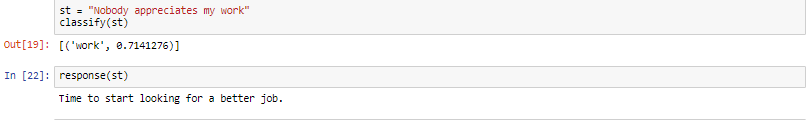
\includegraphics[width=\linewidth]{screenshots/jupyter-notebook/response.png}
    \caption{Jupyter Notebook - Sample Response}
\end{figure}

Greater the expanse and variety of dataset, better the training and furnishing of responses.

\subsubsection{Proposed Headway}

The current training scenario has two parameters:
\begin{itemize}
    \item Number of Epochs
    \item Batch Size
\end{itemize}

\paragraph{Increasing the Number of Epochs}

By maintaining a constant Batch Size of 8, we gradually increment the Number of Epochs.

\begin{figure}[H]
    \centering
    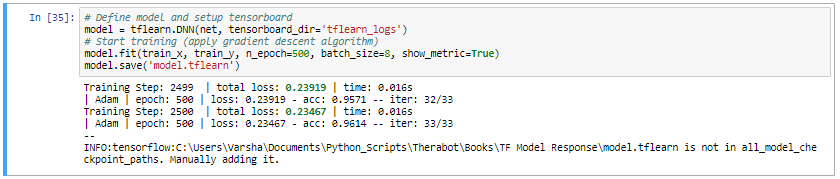
\includegraphics[width=\linewidth]{screenshots/jupyter-notebook/nb-epoch-500.png}
    \caption{Jupyter Notebook - Number of Epochs = 500}
\end{figure}

\begin{figure}[H]
    \centering
    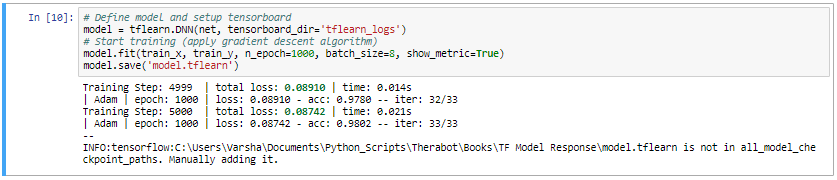
\includegraphics[width=\linewidth]{screenshots/jupyter-notebook/nb-epoch-1000.png}
    \caption{Jupyter Notebook - Number of Epochs = 1000}
\end{figure}

\begin{figure}[H]
    \centering
    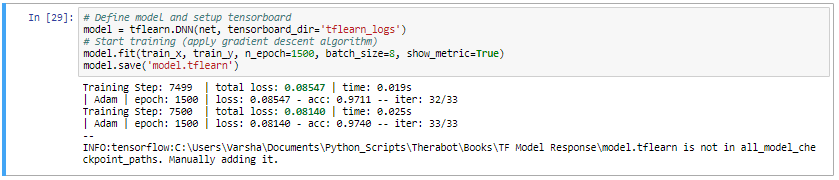
\includegraphics[width=\linewidth]{screenshots/jupyter-notebook/nb-epoch-1500.png}
    \caption{Jupyter Notebook - Number of Epochs = 1500}
\end{figure}

\begin{figure}[H]
    \centering
    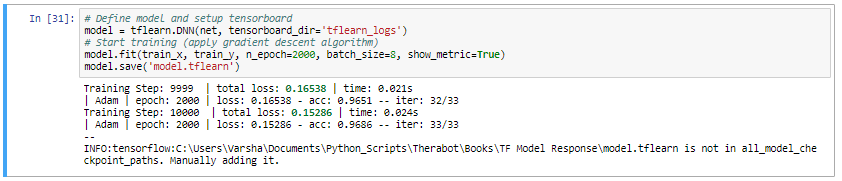
\includegraphics[width=\linewidth]{screenshots/jupyter-notebook/nb-epoch-2000.png}
    \caption{Jupyter Notebook - Number of Epochs = 2000}
\end{figure}

\begin{center}
    \begin{tabular}{ |c|c|c| } 
        \hline
        Number of Epochs & Loss Incurred & Accuracy \\ [0.5ex]
        \hline\hline
        500 & 0.23467 & 0.9614 \\
        1000 & 0.08742 & 0.9802 \\
        1500 & 0.08140 & 0.9740 \\
        2000 & 0.15286 & 0.9686 \\
        2250 & 0.20507 & 0.9544 \\
        2456(~2500) & 0.27993 & 0.9525 \\
        \hline
    \end{tabular}
\end{center}

The outcome of any DNN model is two things. First, it should return the desired response precisely. Second, the loss at each iteration during training must be optimized. From the above table, it is evident that by increasing the batch size the losses are reduced.

But we do observe that when the \texttt{n\_epoch = 2000}, the losses increase. This is the case of overfitting the data. It means that your model does not learn the data, it memorizes the data. You have to find the accuracy of validation data for each epoch or maybe iteration to investigate whether it over-fits or not. To deal with this problem, another approaches are used for avoiding the problem. Adding noise to different parts of models, like drop out or somehow batch normalization with a moderated batch size, help these learning algorithms not to over-fit even after so many epochs.

Since, accuracy is the prime factor, our model works at \textbf{n\_epoch = 1000} with a \textbf{very high accuracy of 0.98}.

\paragraph{Increasing the Batch Size}

By maintaining the number of epochs at 1000, we increase the batch size.

\begin{figure}[H]
    \centering
    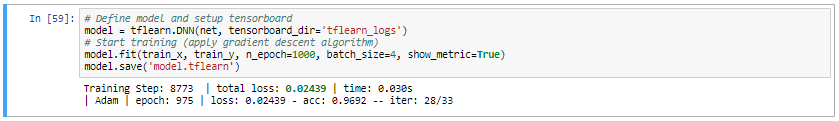
\includegraphics[width=\linewidth]{screenshots/jupyter-notebook/batch-size-4.png}
    \caption{Jupyter Notebook - Batch Size = 4}
\end{figure}

\begin{figure}[H]
    \centering
    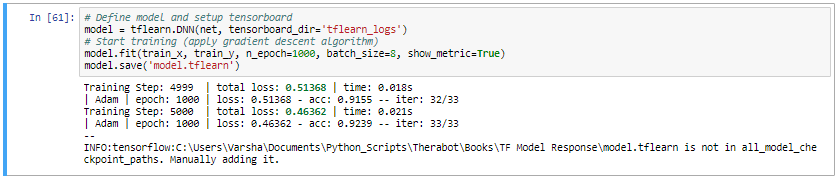
\includegraphics[width=\linewidth]{screenshots/jupyter-notebook/batch-size-8.png}
    \caption{Jupyter Notebook - Batch Size = 8}
\end{figure}

\begin{figure}[H]
    \centering
    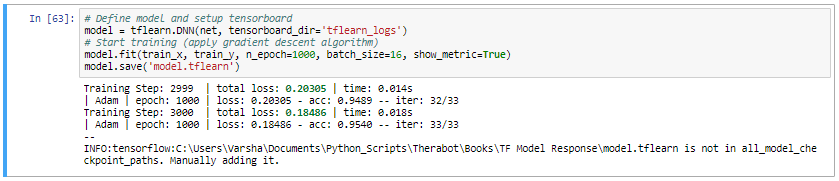
\includegraphics[width=\linewidth]{screenshots/jupyter-notebook/batch-size-16.png}
    \caption{Jupyter Notebook - Batch Size = 16}
\end{figure}

\begin{figure}[H]
    \centering
    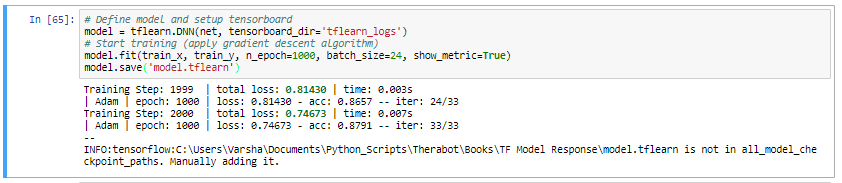
\includegraphics[width=\linewidth]{screenshots/jupyter-notebook/batch-size-24.png}
    \caption{Jupyter Notebook - Batch Size = 24}
\end{figure}

\begin{figure}[H]
    \centering
    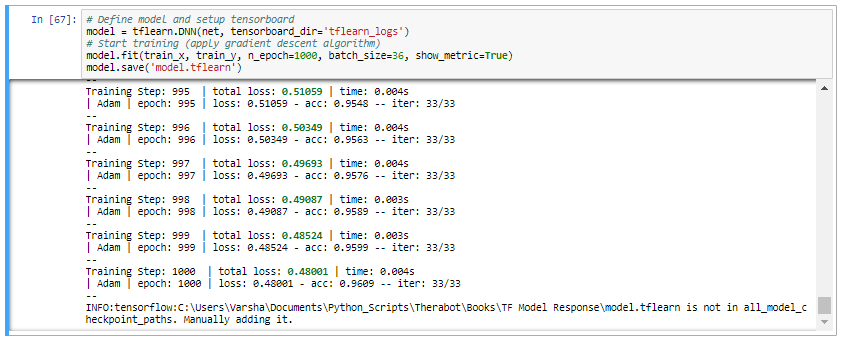
\includegraphics[width=\linewidth]{screenshots/jupyter-notebook/batch-size-36.png}
    \caption{Jupyter Notebook - Batch Size = 36}
\end{figure}

\begin{center}
    \begin{tabular}{ |c|c|c| } 
        \hline
        Batch Size & Loss Incurred & Accuracy \\ [0.5ex]
        \hline\hline
        4 & 0.02439 & 0.9692 \\
        8 & 0.46362 & 0.9239 \\
        16 & 0.18486 & 0.9540 \\
        24 & 0.74673 & 0.8791 \\
        36 & 0.48001 & 0.9609 \\
        48 & 0.83720 & 0.8264 \\
        \hline
    \end{tabular}
\end{center}

On deeper analysis of the results, we understand that by increasing the batch\_size we approach the case of overfitting the data. Hence, nest accuracy is obtained when the batch size is 8(or 16) for most of the given kinds of dataset.

\pagebreak

\section{Screenshots}

\subsection{Website}

\noindent
Below are some screenshots of the website, which is hosted on the cloud. It is a Progressive Web App (PWA), meaning it can function as a functioning native Android/iOS application or a desktop web application on the same code.

\vspace*{\fill}
\begin{figure}[H]
    \centering
    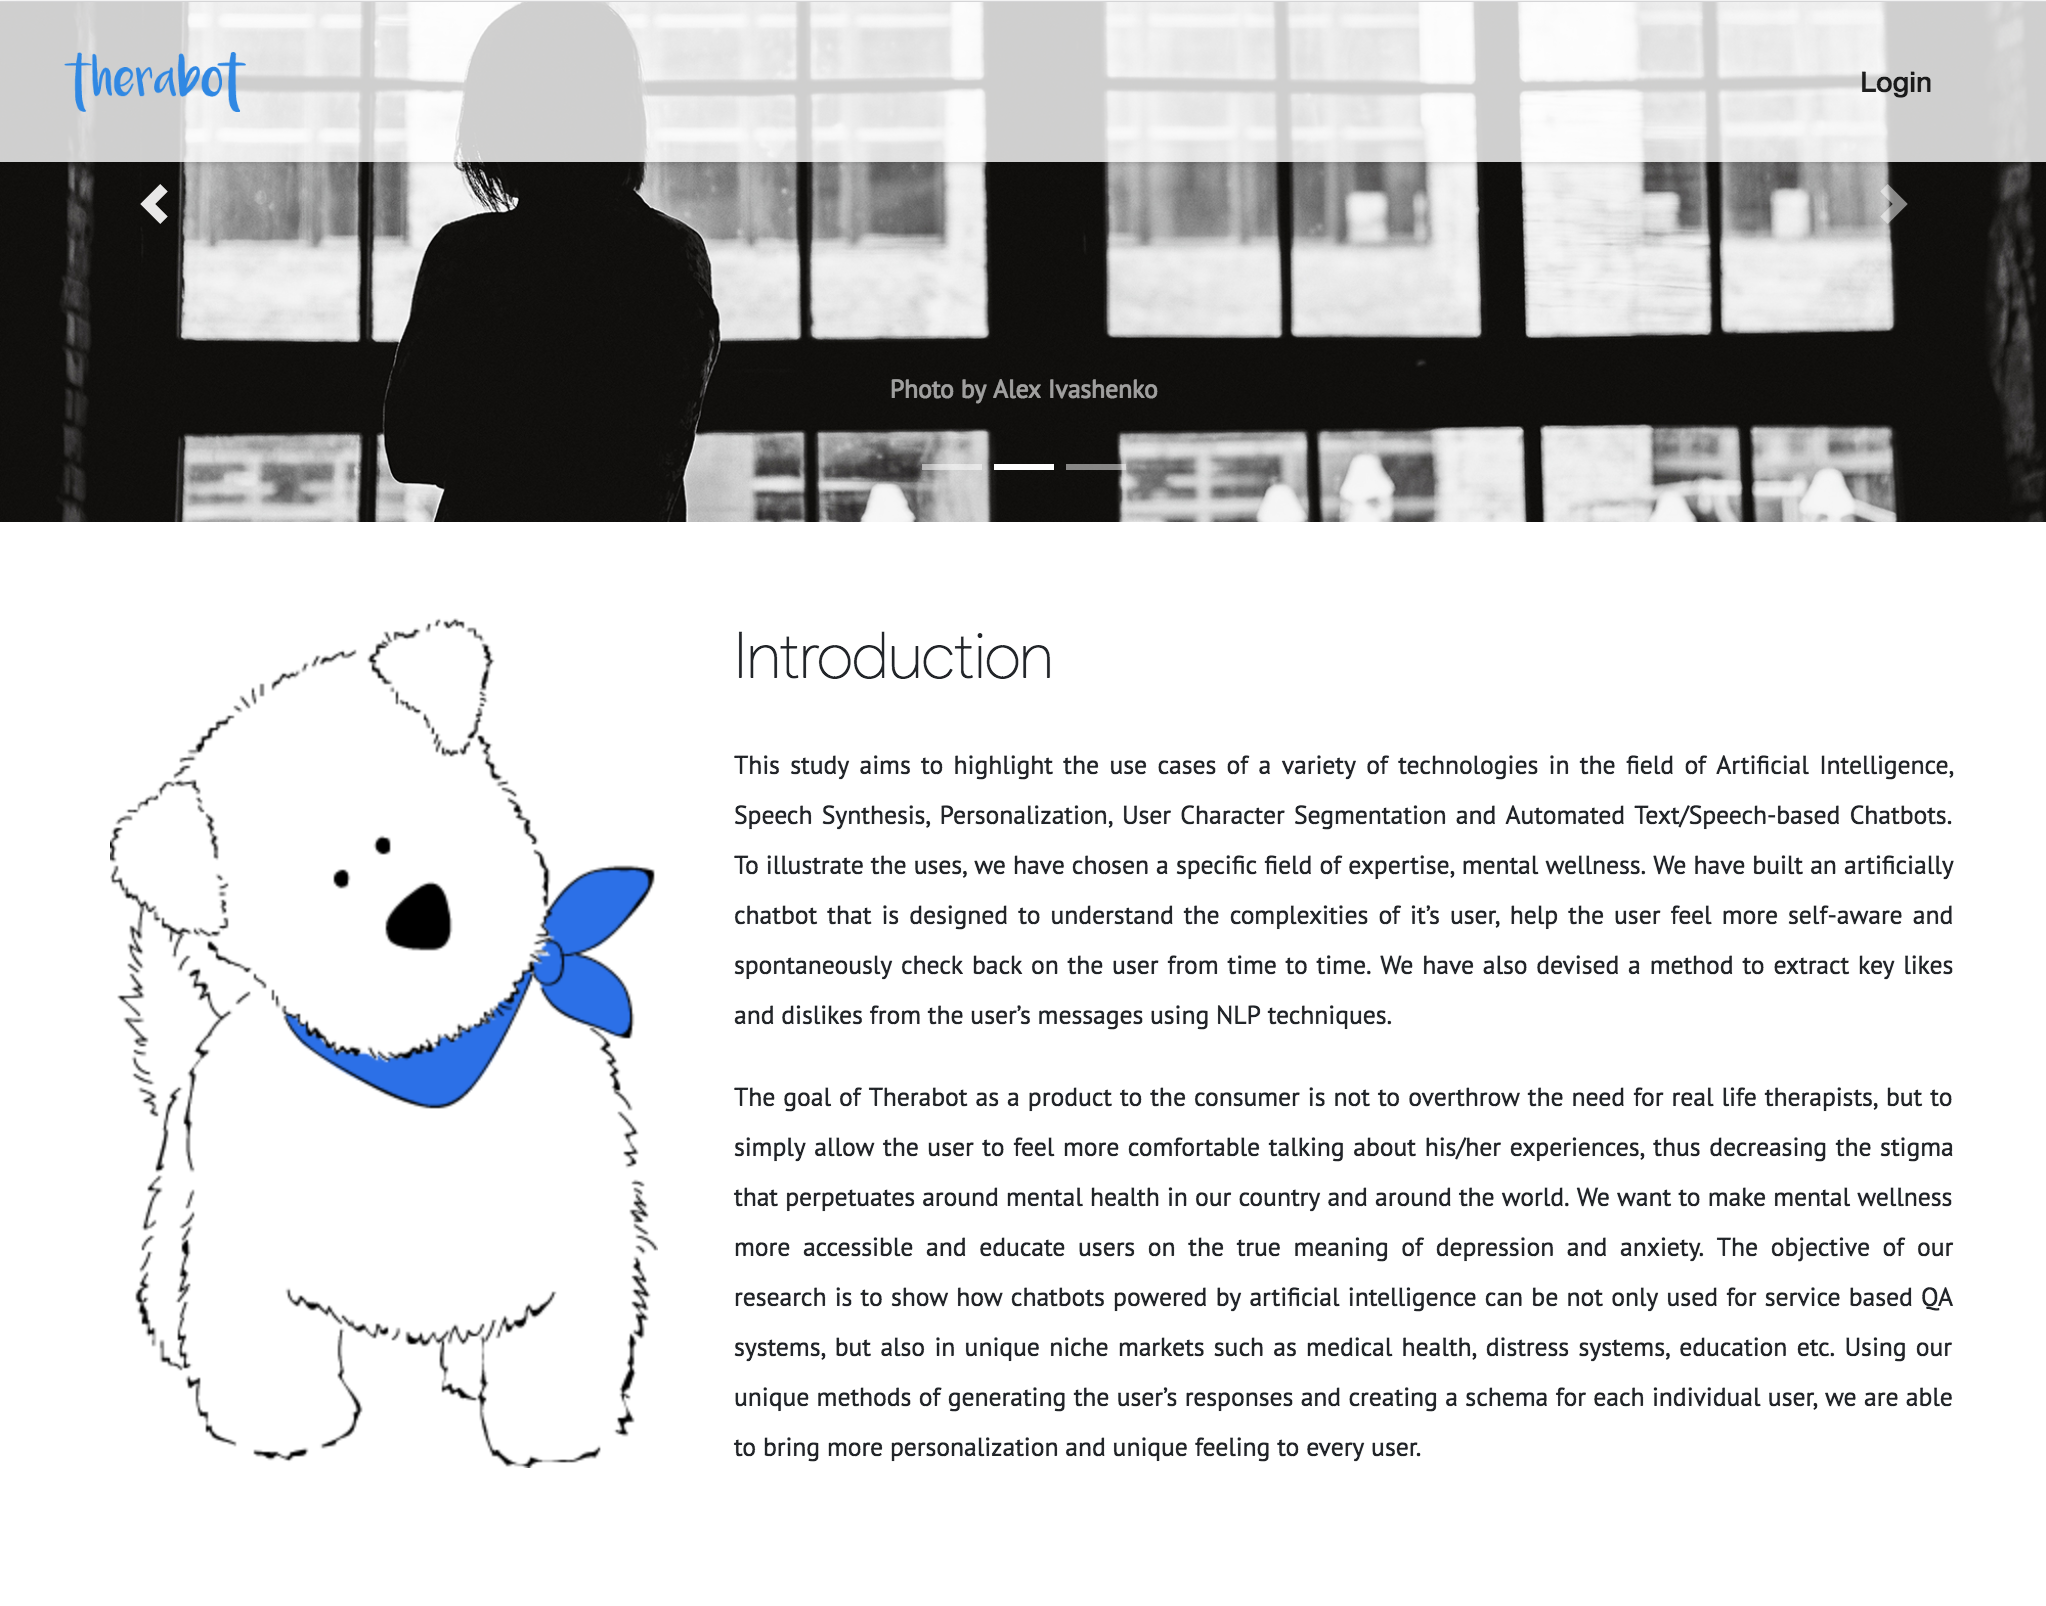
\includegraphics[width=\linewidth]{screenshots/website/website-introduction.png}
    \caption{Introduction}
\end{figure}
\vspace*{\fill}

\pagebreak

\vspace*{\fill}
\begin{figure}[H]
    \centering
    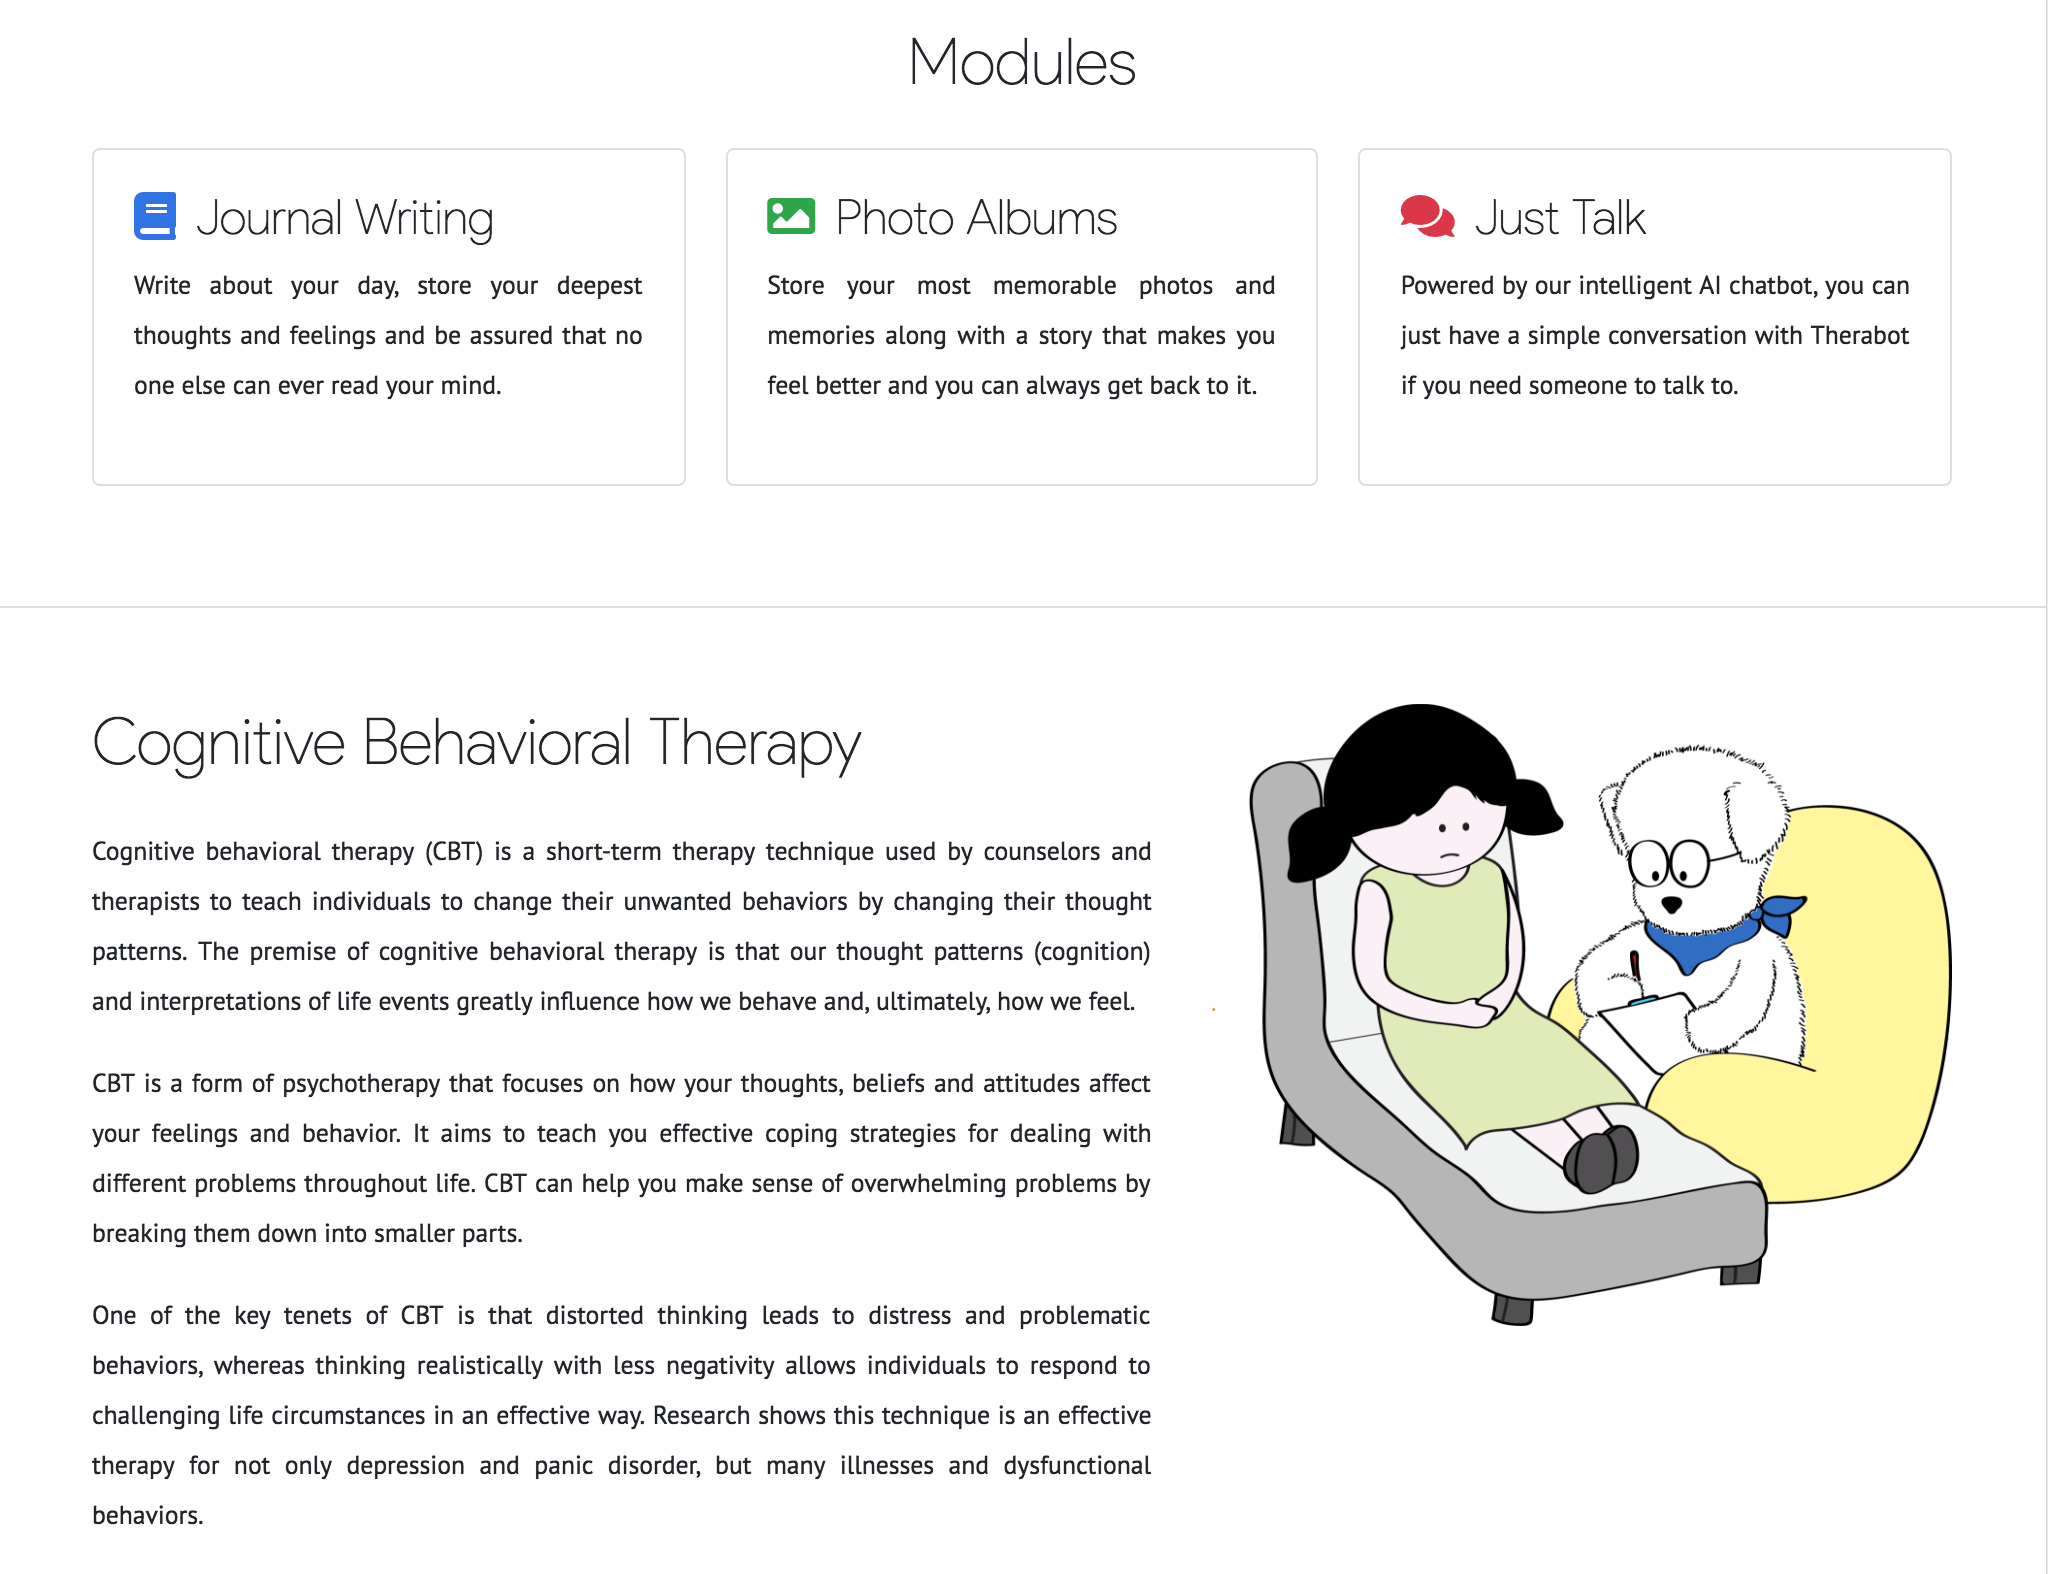
\includegraphics[width=\textwidth]{screenshots/website/website-cbt.png}
    \caption{Cognitive Behavioral Therapy}
\end{figure}

\begin{figure}[H]
    \centering
    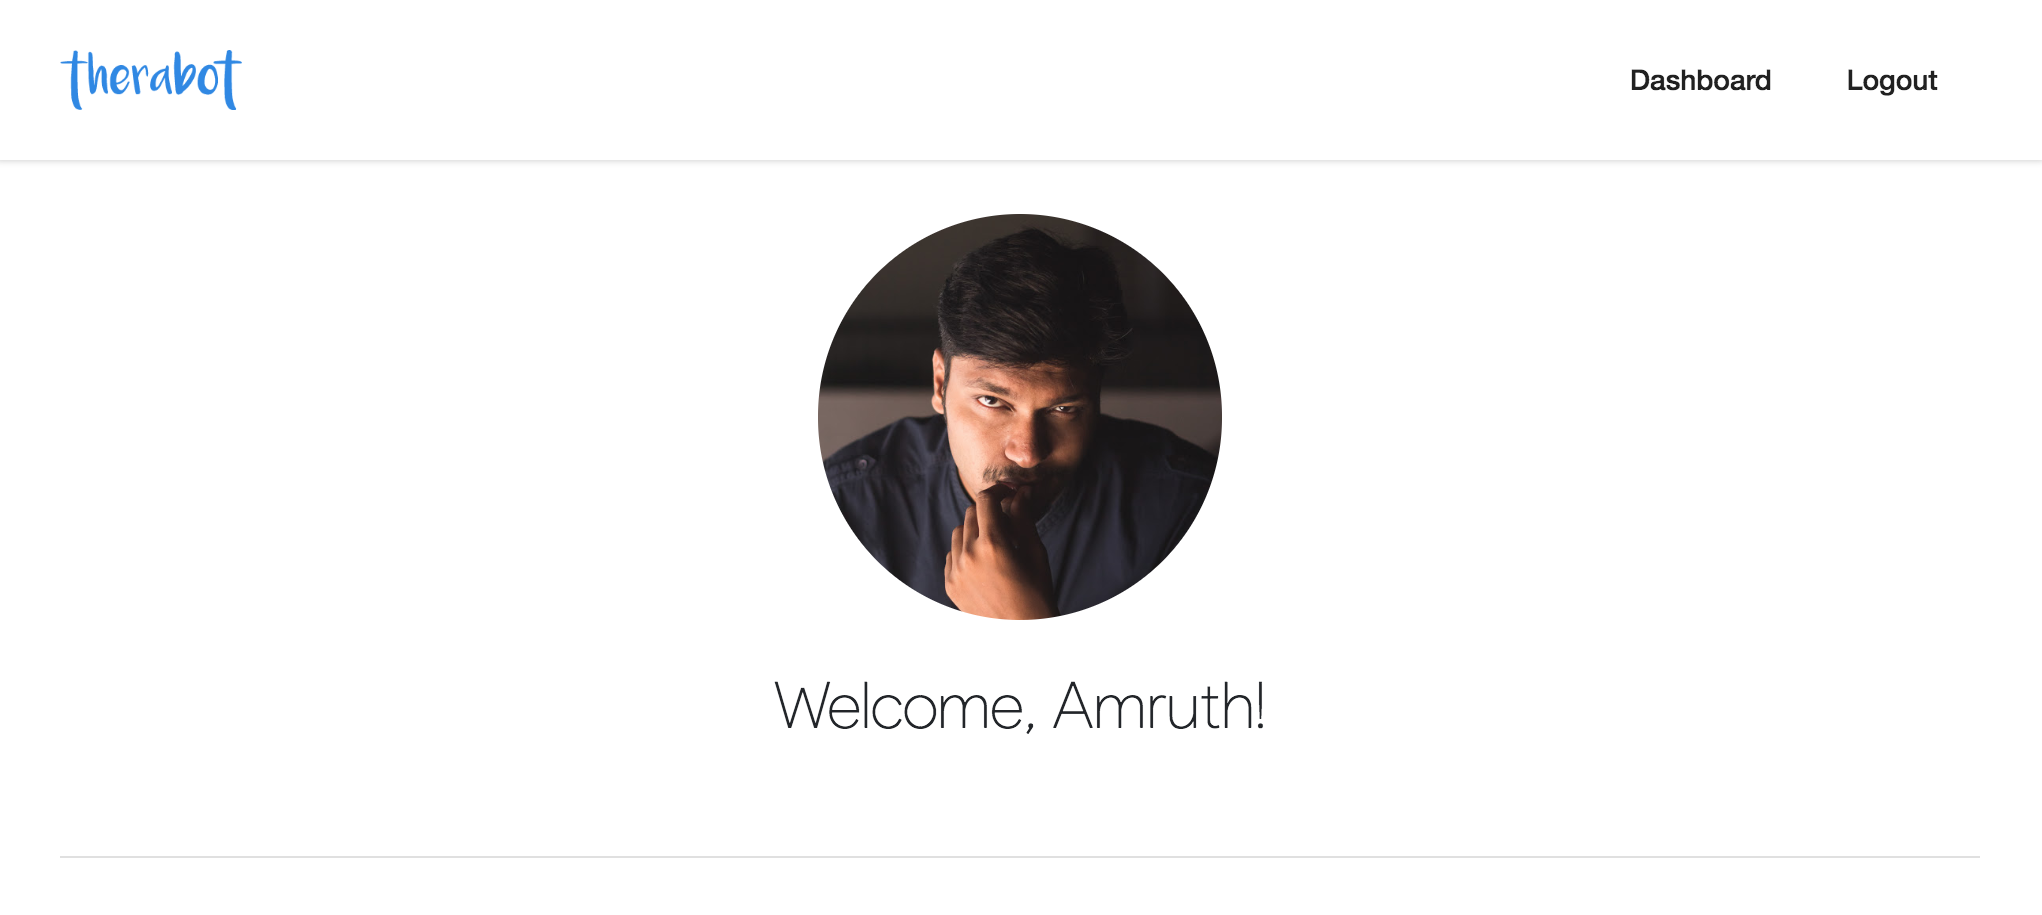
\includegraphics[width=\textwidth]{screenshots/website/website-welcome.png}
    \caption{Welcome - User Dashboard}
\end{figure}
\vspace*{\fill}

\pagebreak

\vspace*{\fill}
\begin{figure}[H]
    \centering
    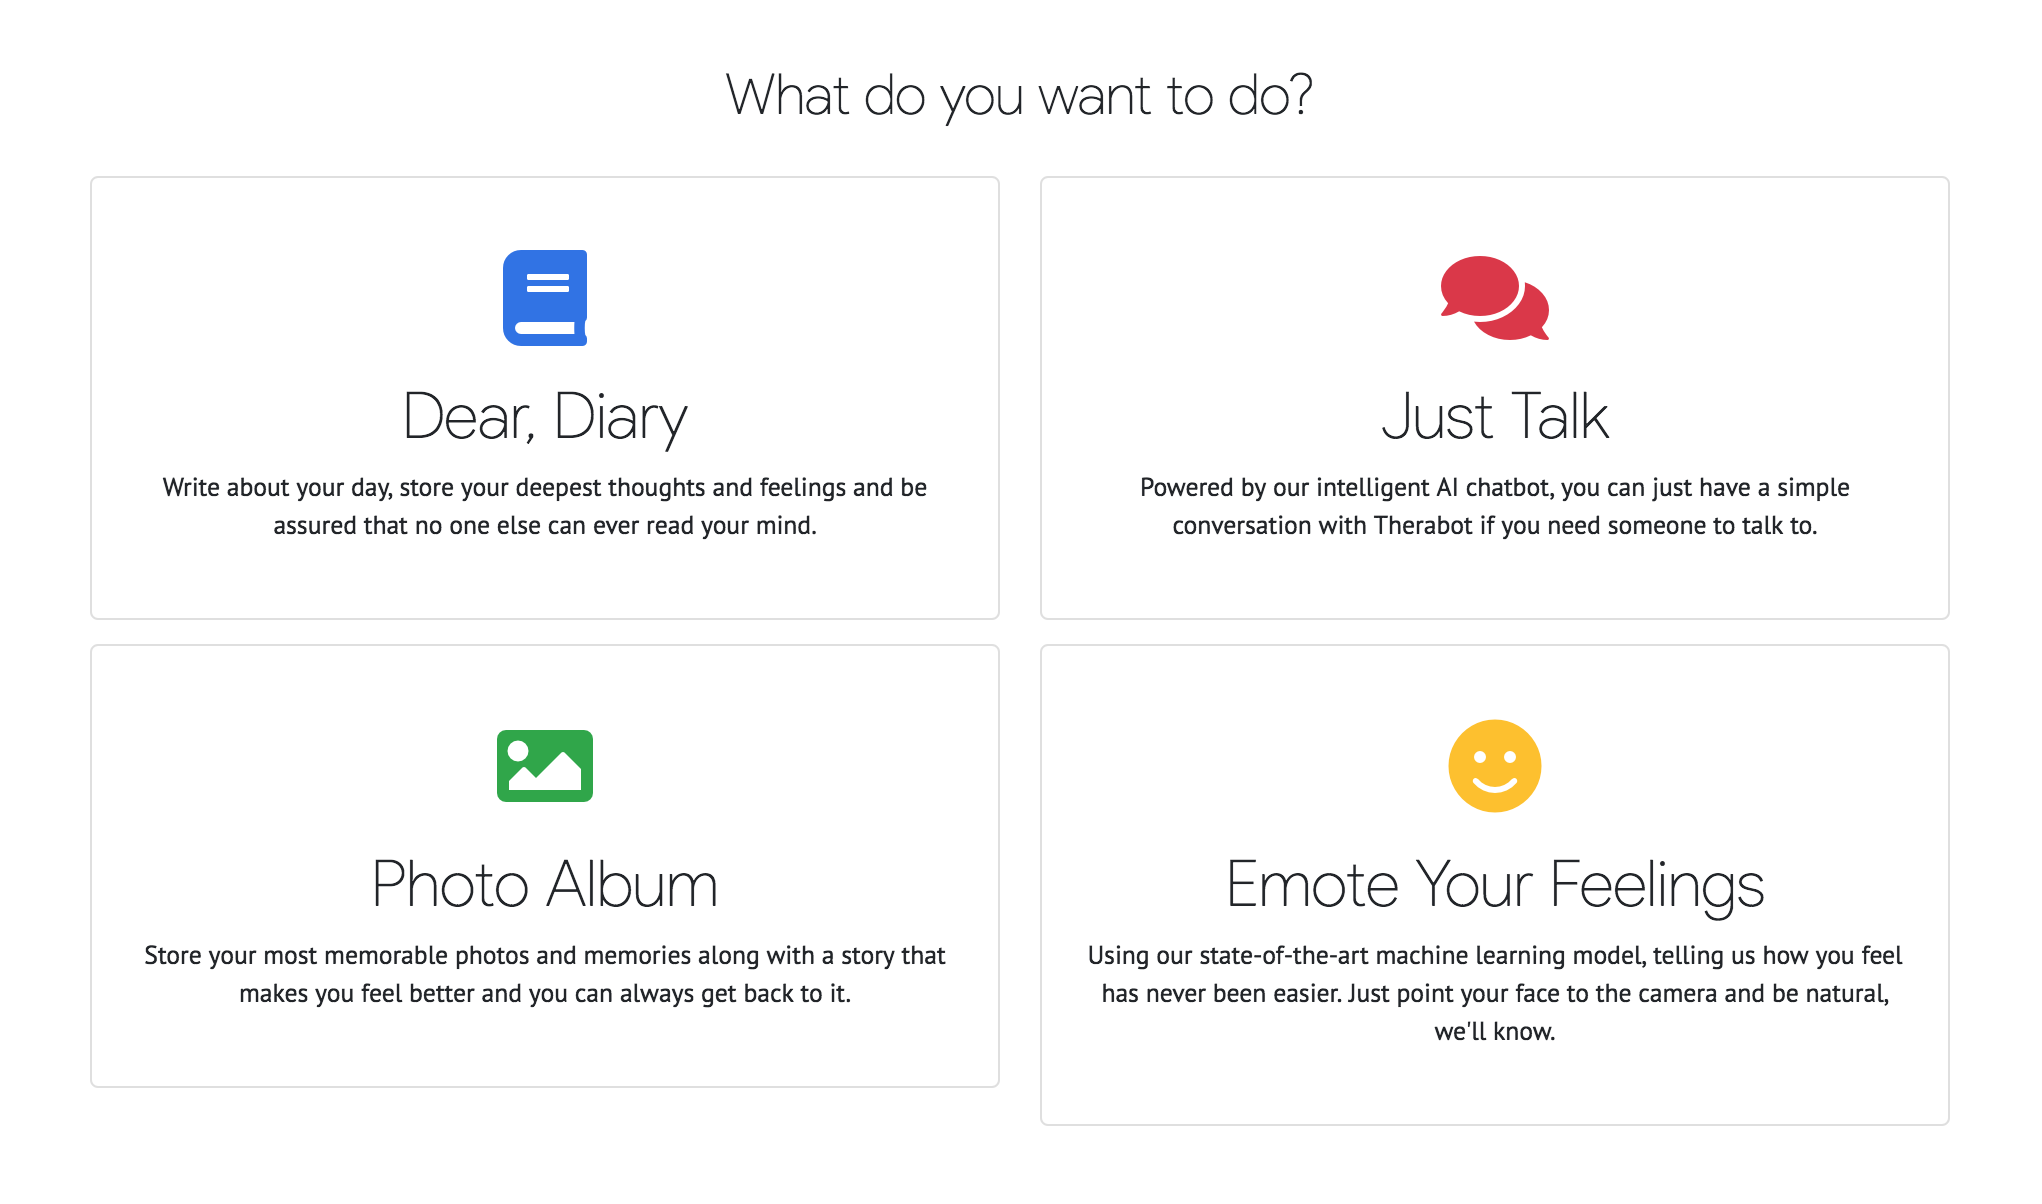
\includegraphics[width=\textwidth]{screenshots/website/website-modules.png}
    \caption{Modules on the Website}
\end{figure}

\begin{figure}[H]
    \centering
    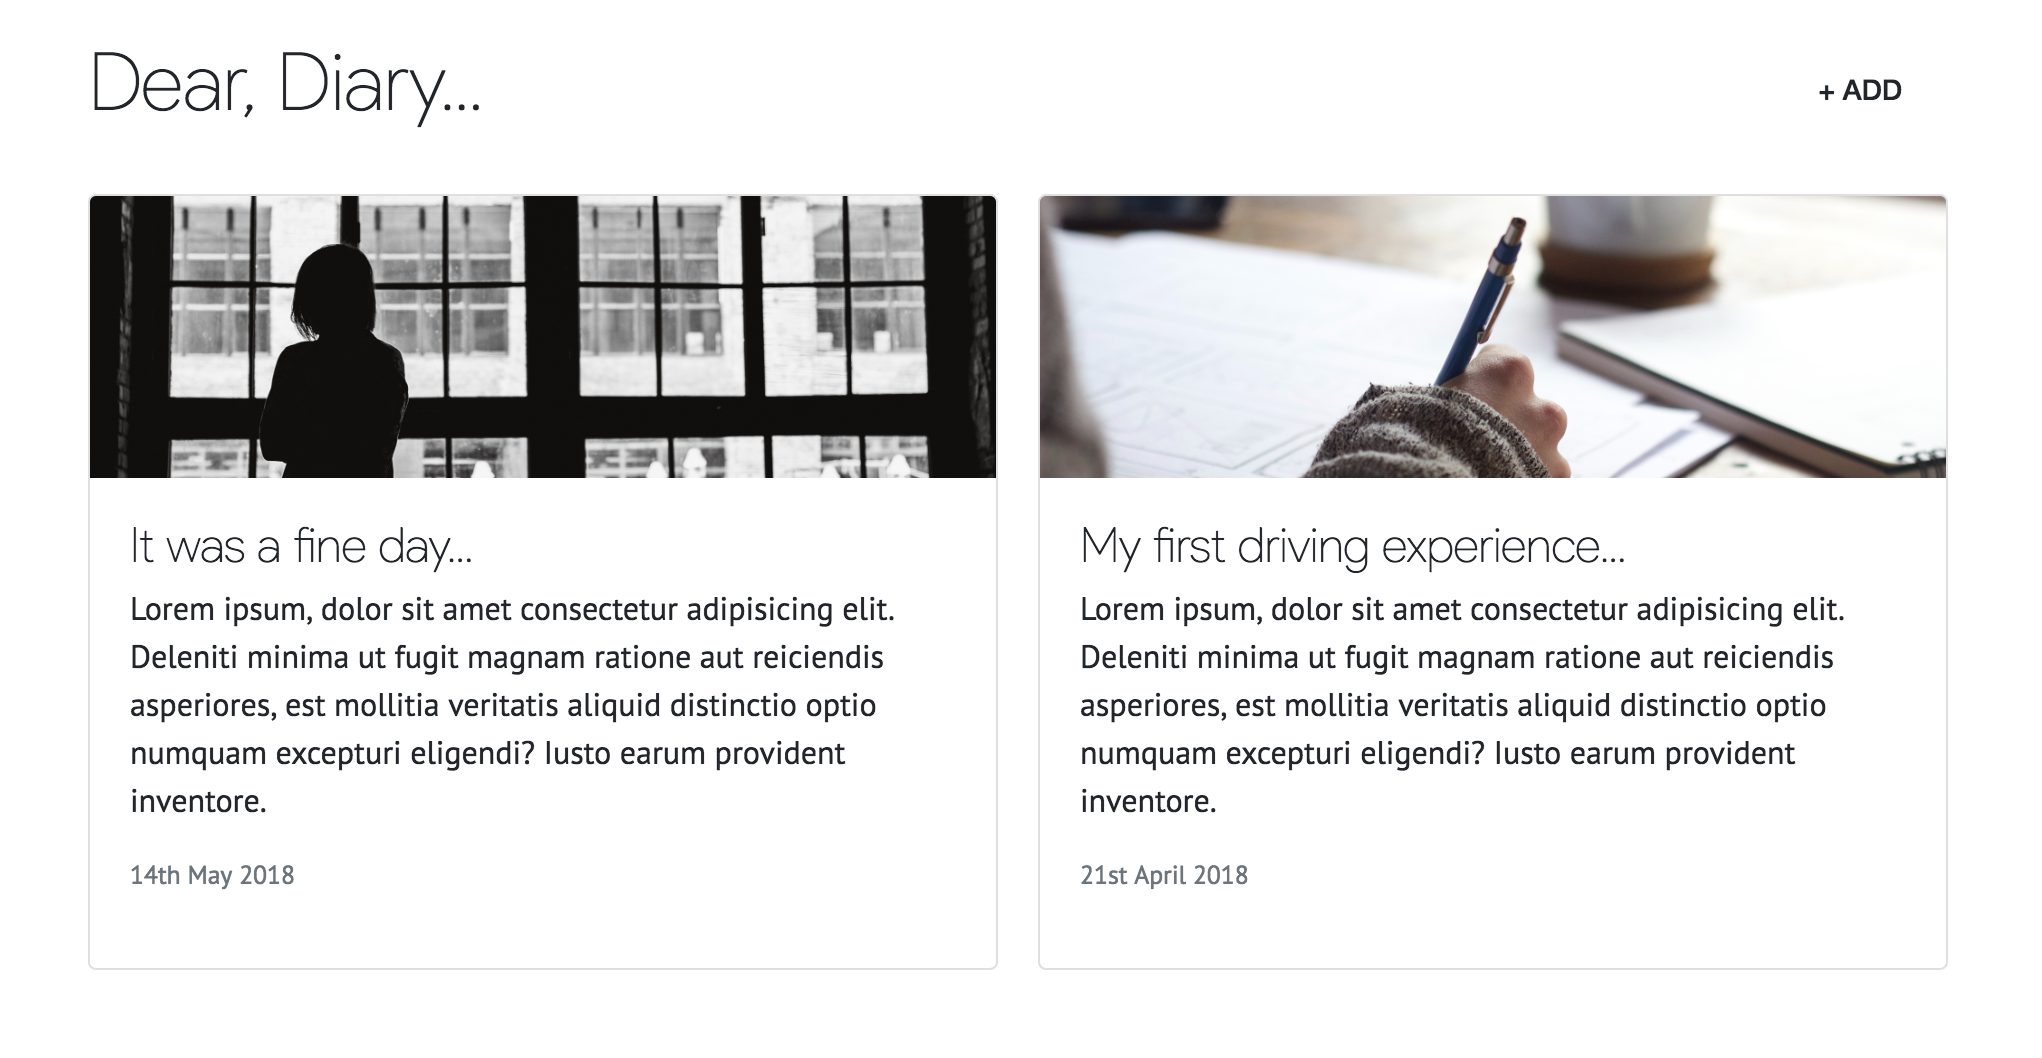
\includegraphics[width=\textwidth]{screenshots/website/website-dear-diary.png}
    \caption{Module \#1 - Dear Diary}
\end{figure}
\vspace*{\fill}

\pagebreak

\vspace*{\fill}
\begin{figure}[H]
    \centering
    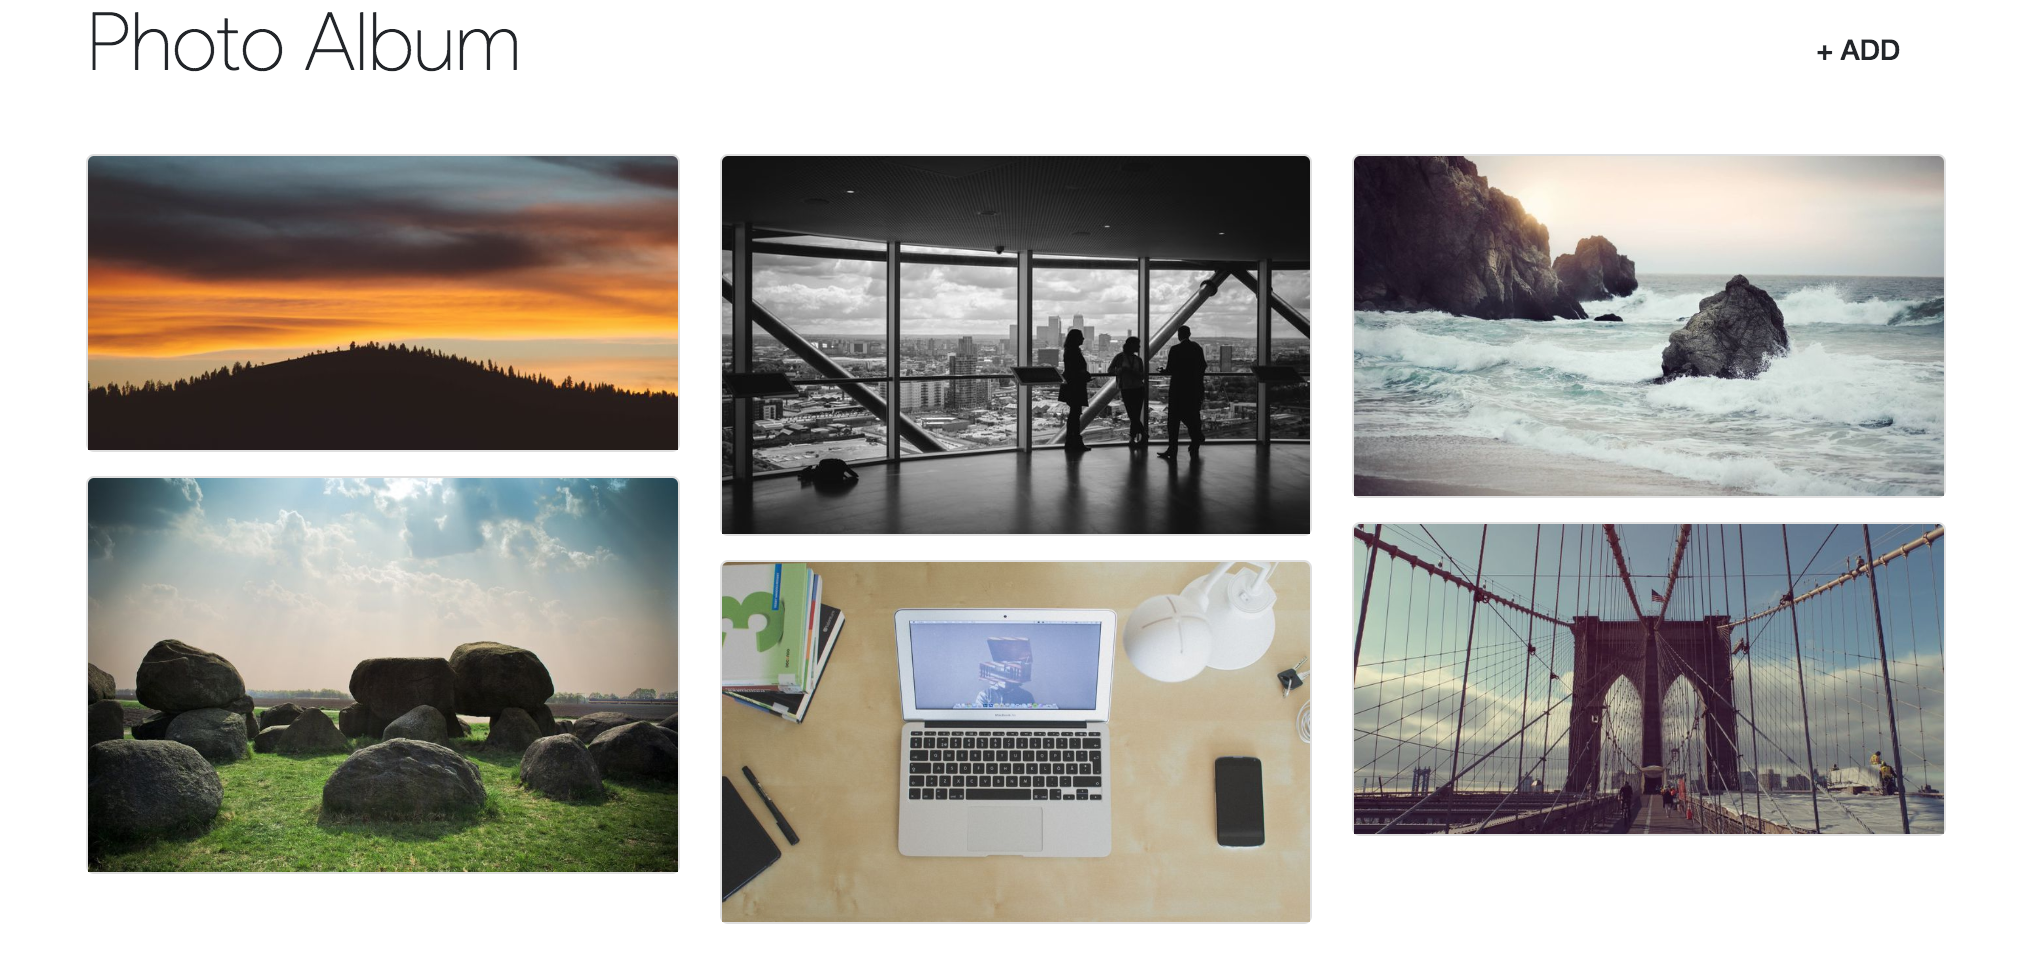
\includegraphics[width=\textwidth]{screenshots/website/website-photo-album.png}
    \caption{Module \#2 - Photo Album}
\end{figure}

\begin{figure}[H]
    \centering
    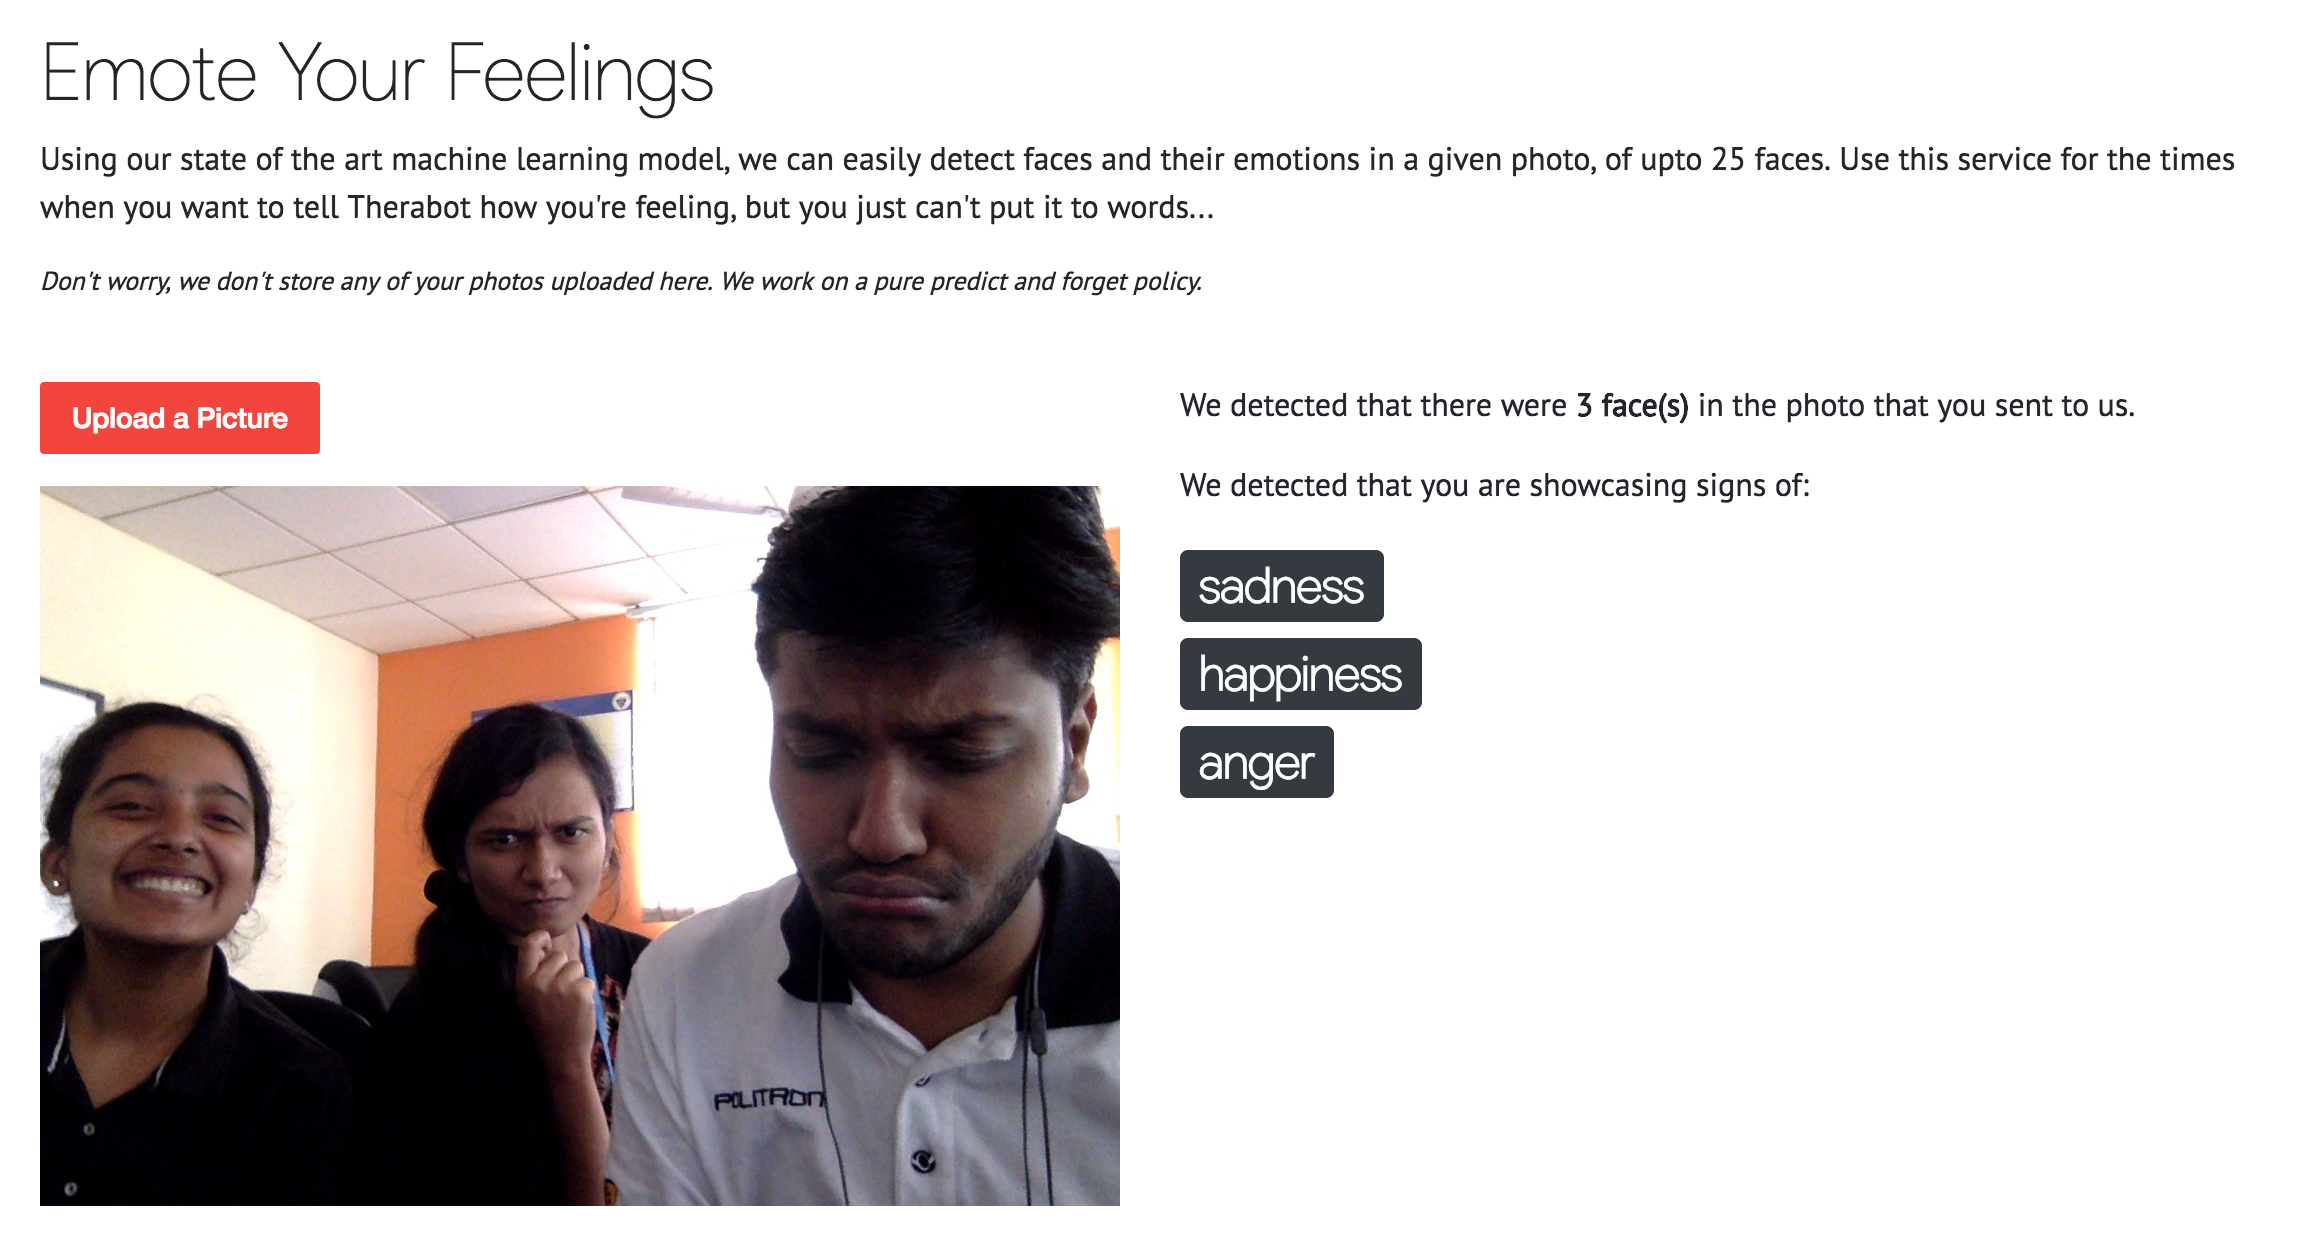
\includegraphics[width=\textwidth]{screenshots/website/website-emote-feelings.png}
    \caption{Module \#3 - Emote your Feelings}
\end{figure}
\vspace*{\fill}

\pagebreak

\subsection{Chatbot}

\noindent
Below are some screenshots of the chatbot, and it’s various conversational trees showcased in action:

\vspace*{\fill}
\begin{figure}[H]
    \centering
    \begin{minipage}{0.45\textwidth}
        \centering
        
\includegraphics[width=0.9\textwidth]{screenshots/chatbot/1.jpg}
        \caption{Facebook Messenger}
    \end{minipage}\hfill
    \begin{minipage}{0.45\textwidth}
        \centering
        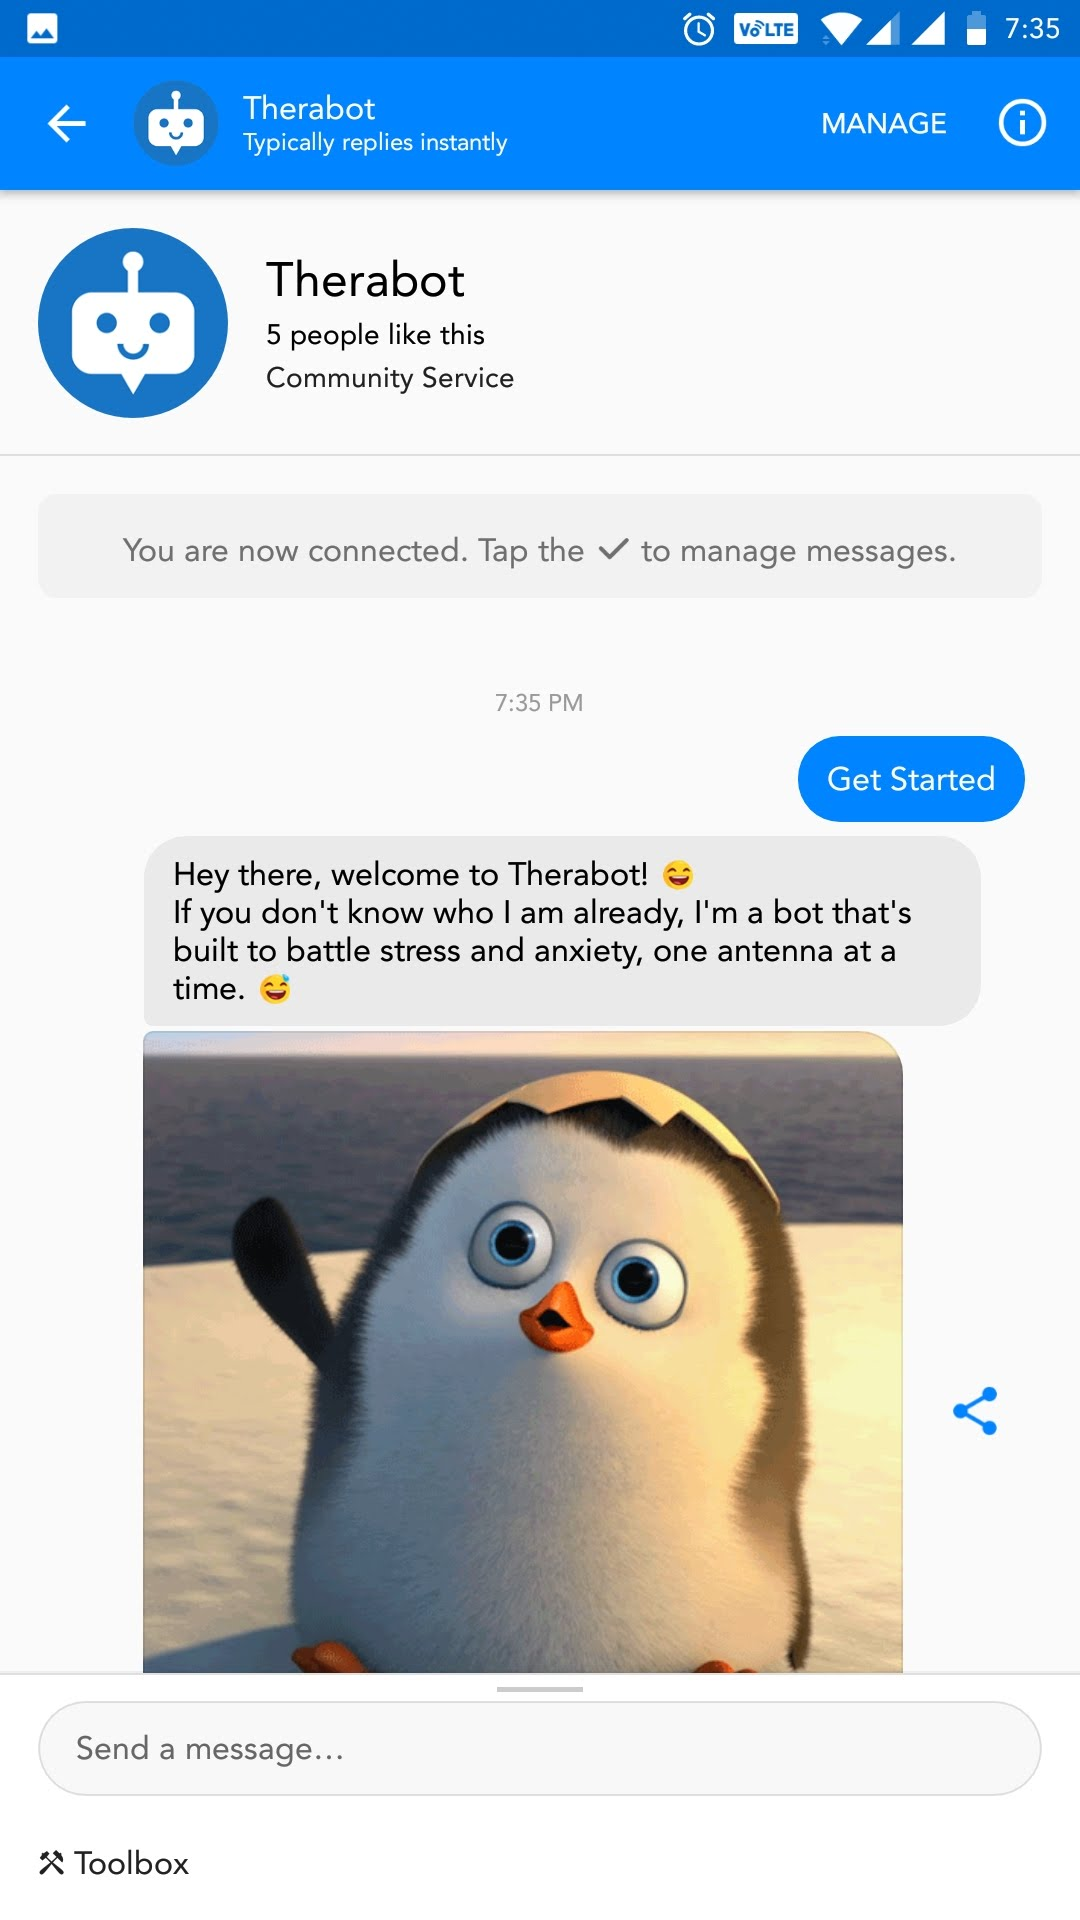
\includegraphics[width=0.9\textwidth]{screenshots/chatbot/2.jpg}
        \caption{User Onboarding}
    \end{minipage}
\end{figure}
\vspace*{\fill}

\pagebreak

\vspace*{\fill}
\begin{figure}[H]
    \centering
    \begin{minipage}{0.45\textwidth}
        \centering
        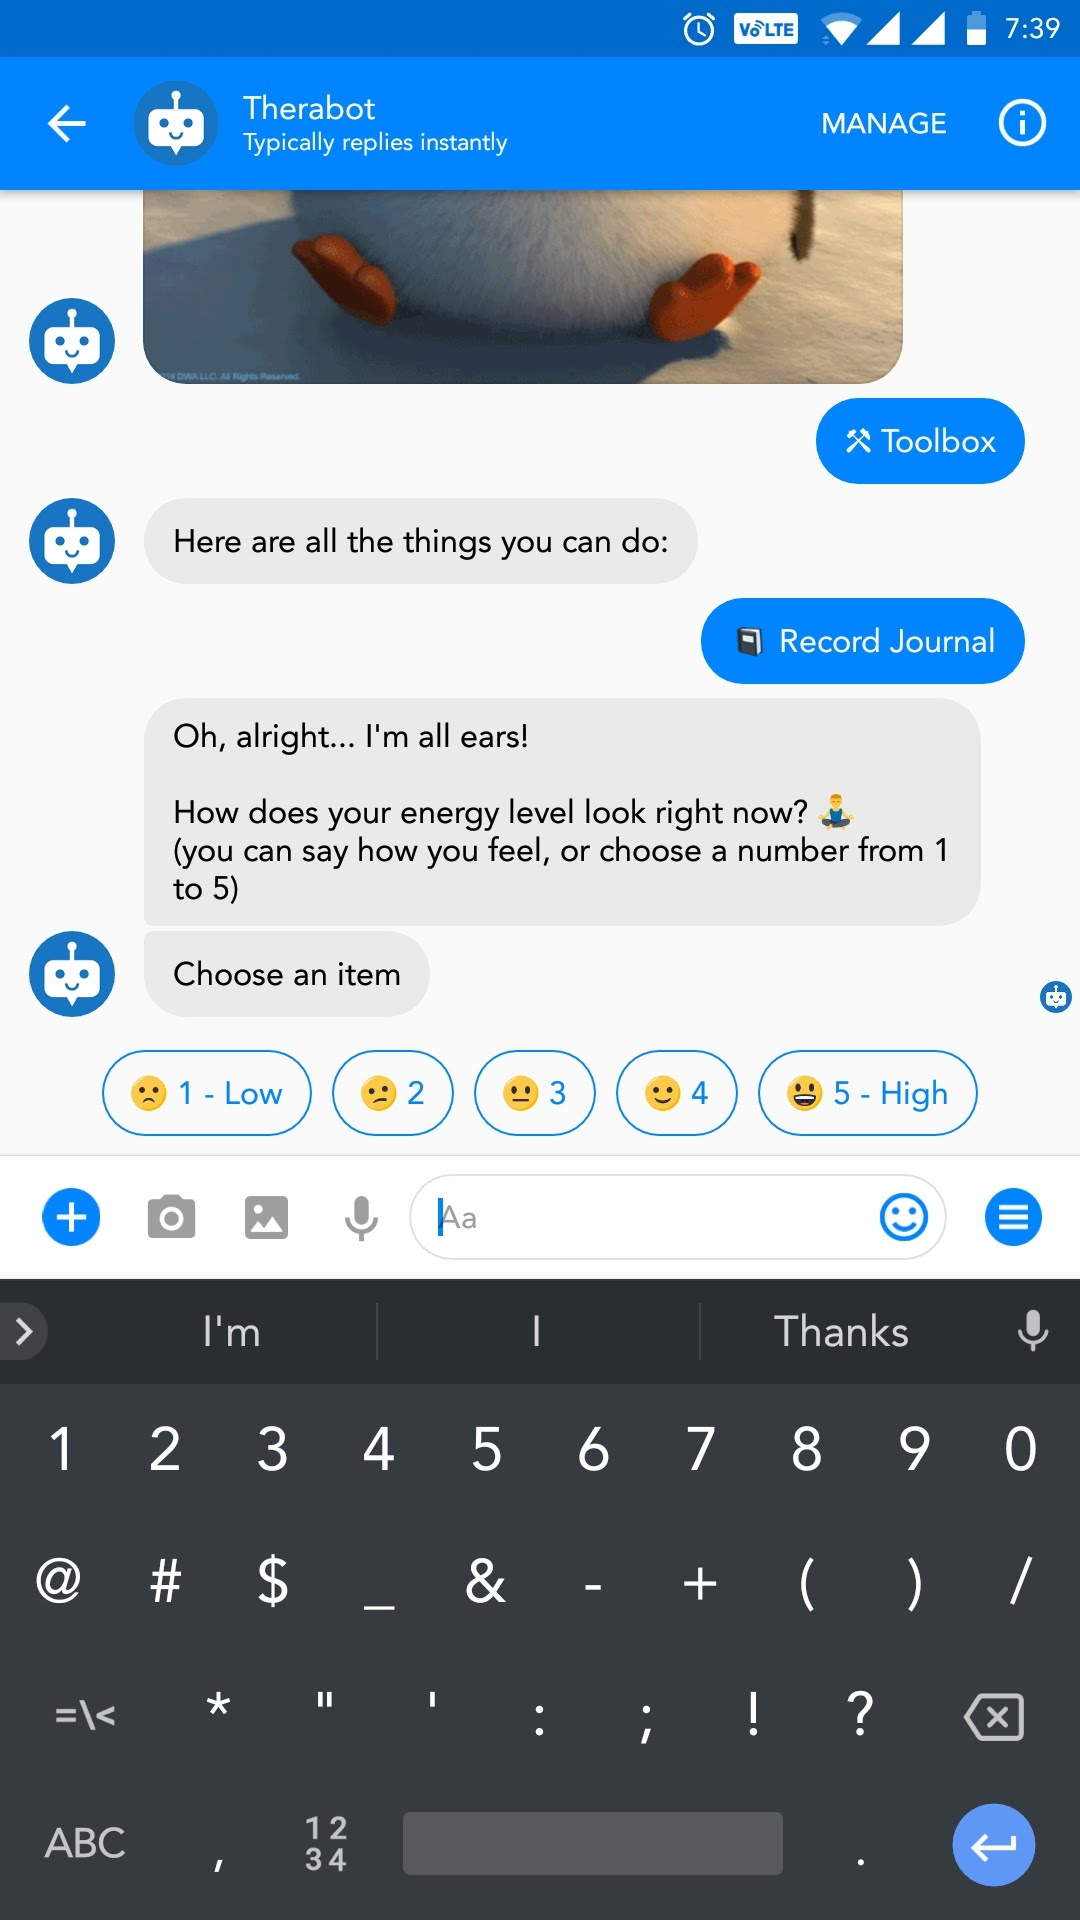
\includegraphics[width=0.9\textwidth]{screenshots/chatbot/3.jpg}
        \caption{Record Journal}
    \end{minipage}\hfill
    \begin{minipage}{0.45\textwidth}
        \centering
        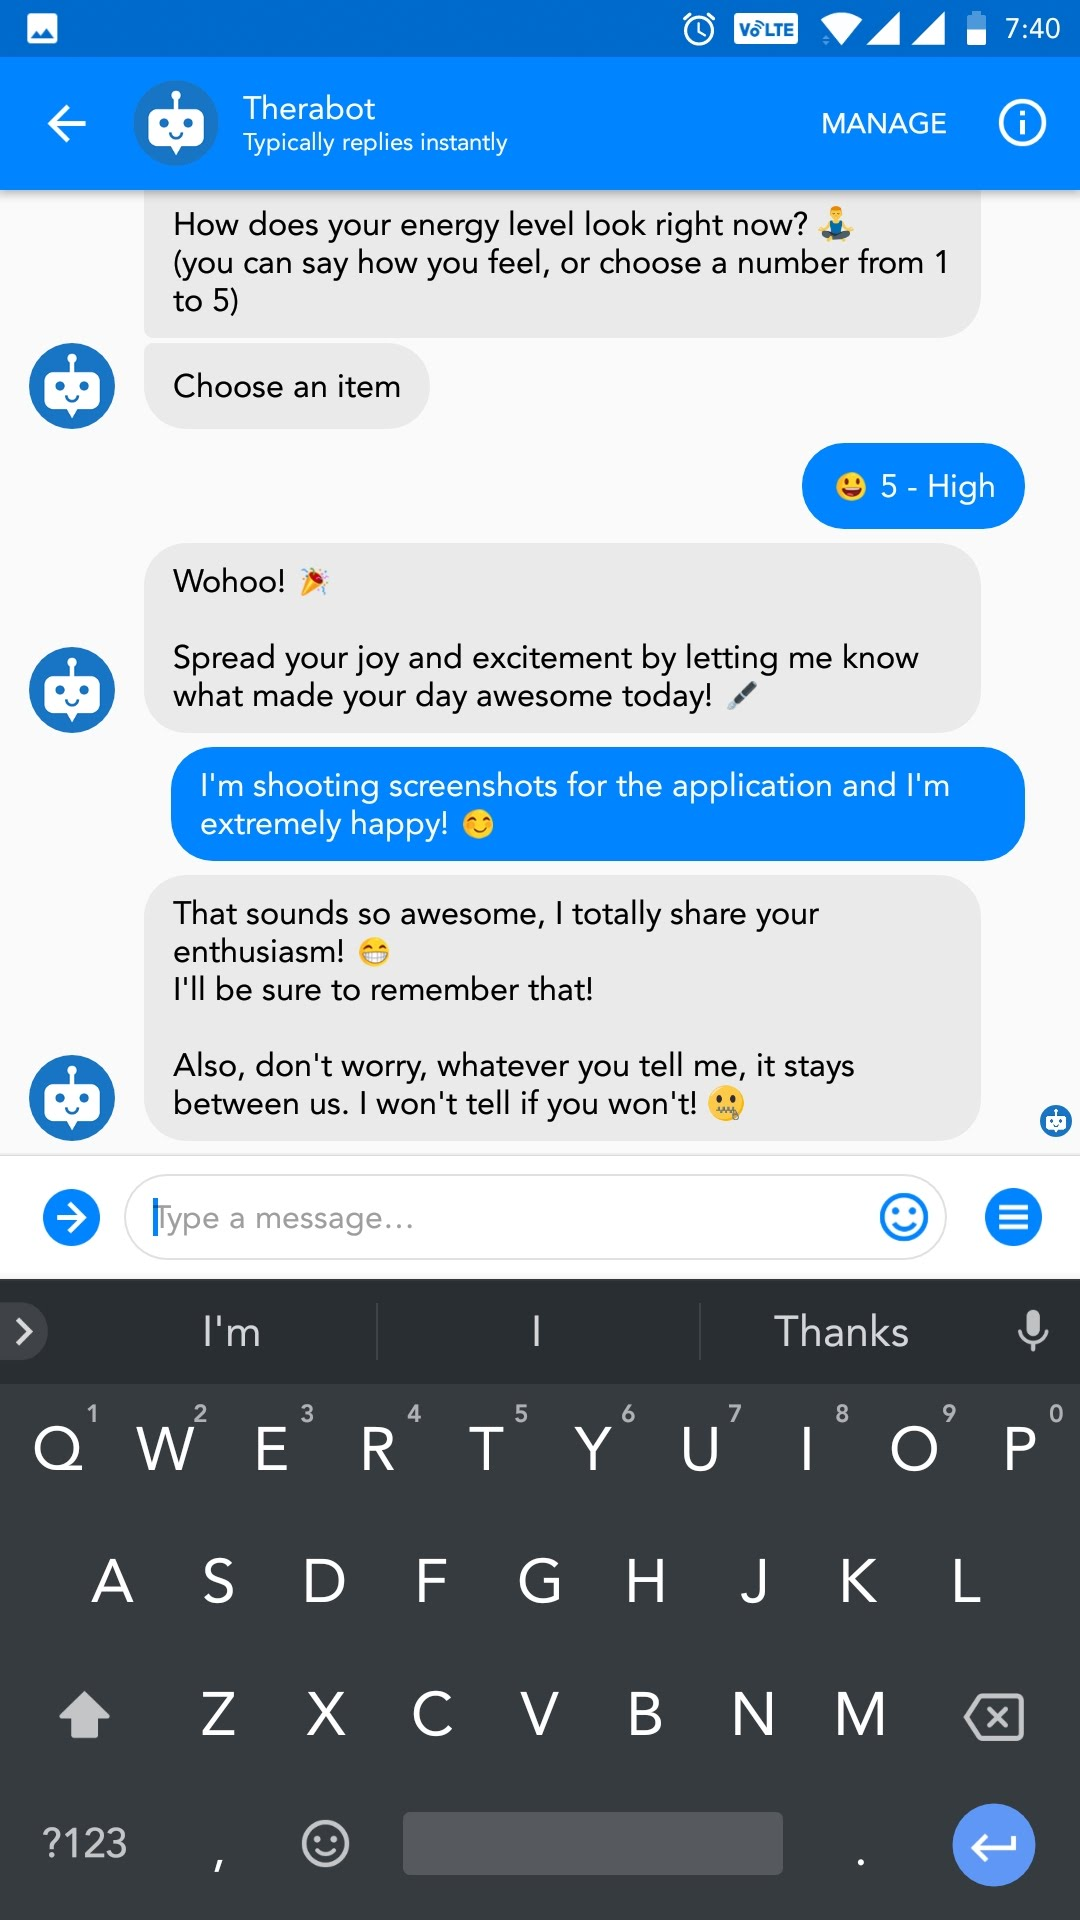
\includegraphics[width=0.9\textwidth]{screenshots/chatbot/4.jpg}
        \caption{Saving Journal Entry}
    \end{minipage}
\end{figure}
\vspace*{\fill}

\pagebreak

\vspace*{\fill}
\begin{figure}[H]
    \centering
    \begin{minipage}{0.45\textwidth}
        \centering
        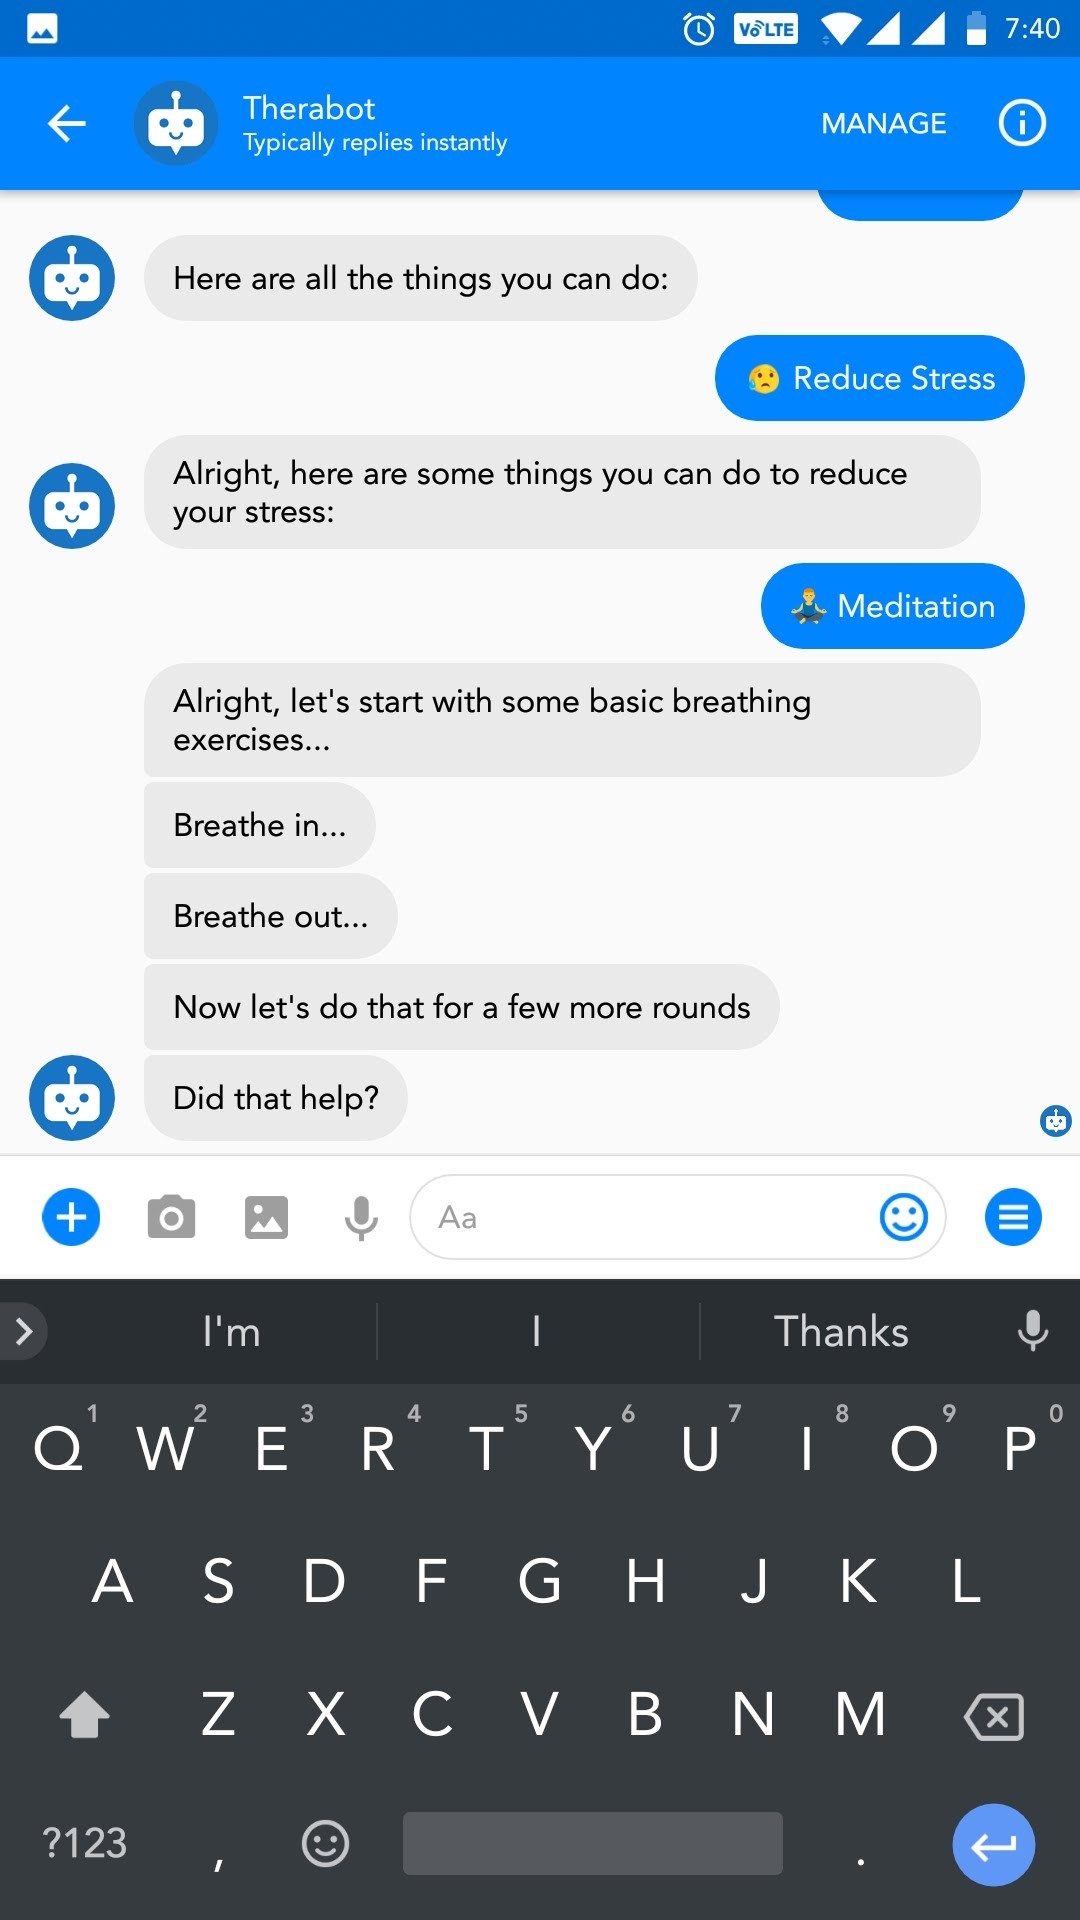
\includegraphics[width=0.9\textwidth]{screenshots/chatbot/5.jpg}
        \caption{Meditation}
    \end{minipage}\hfill
    \begin{minipage}{0.45\textwidth}
        \centering
        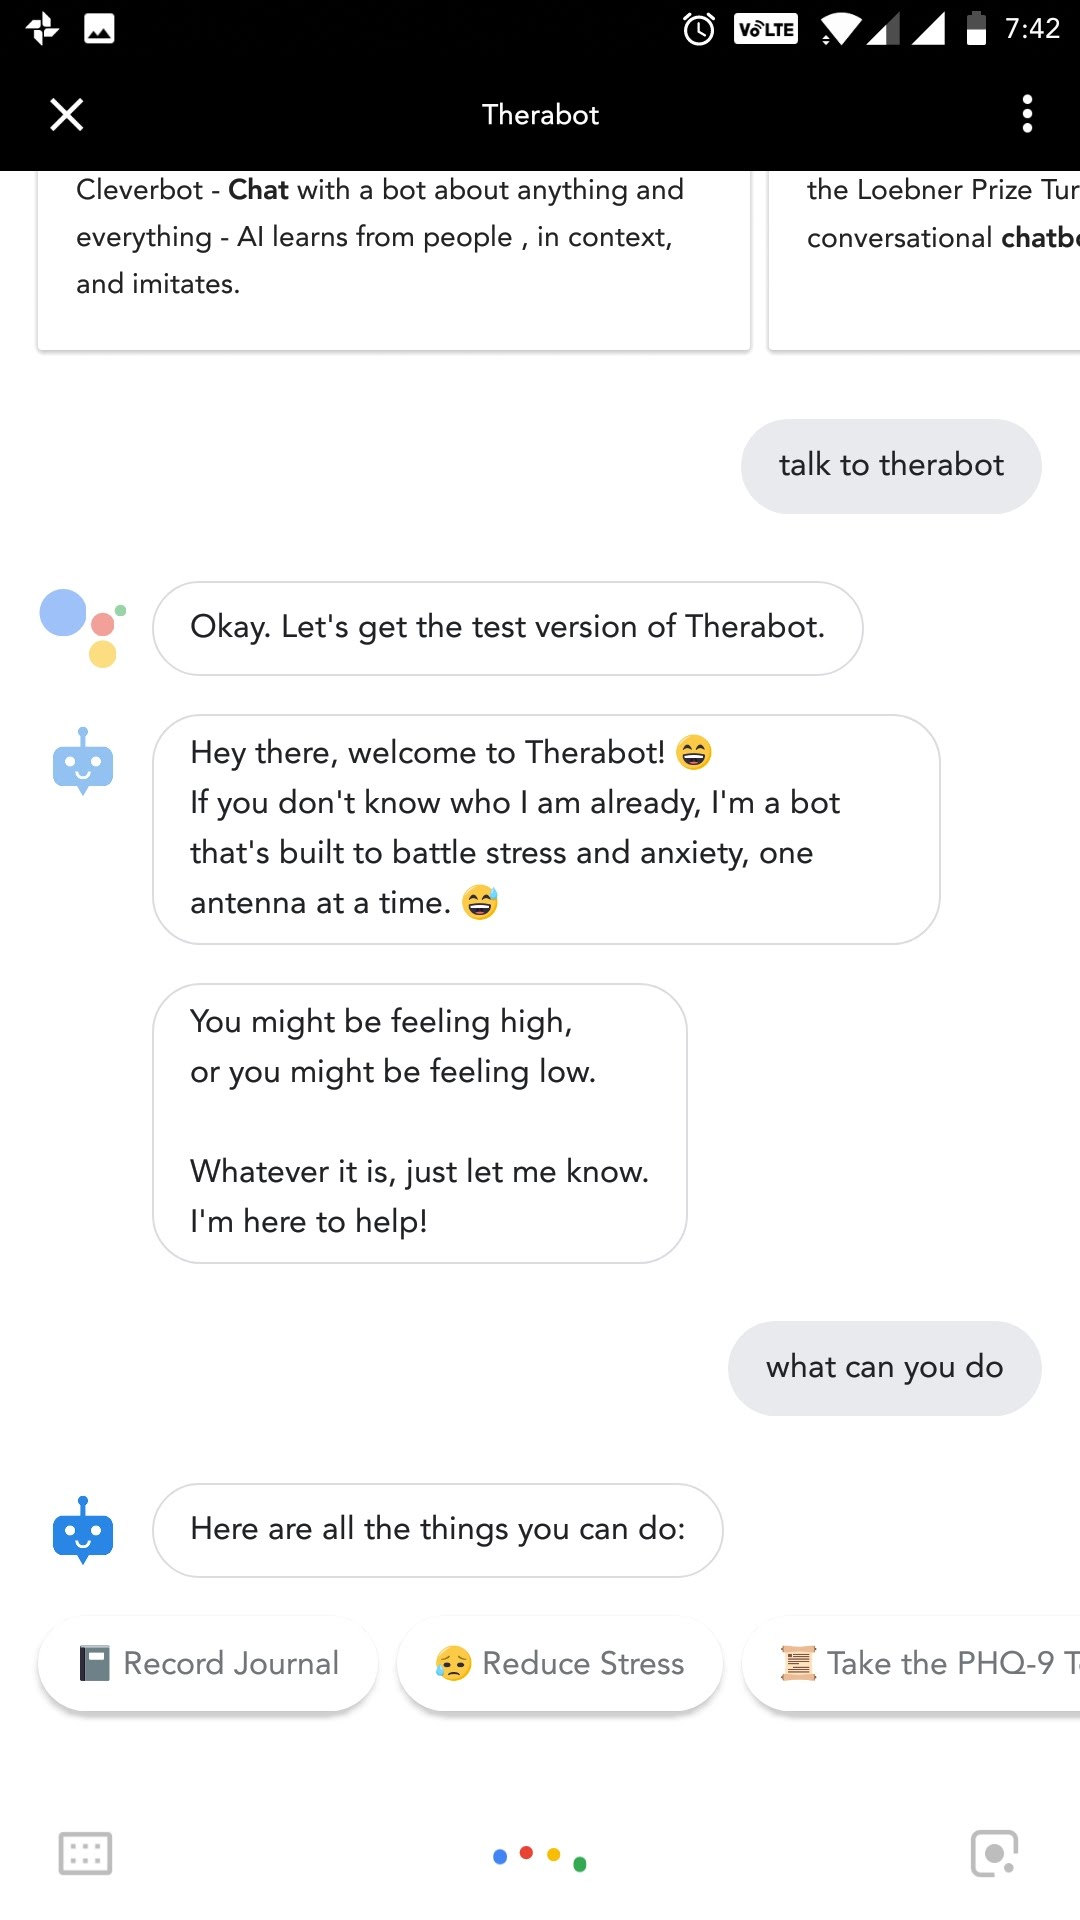
\includegraphics[width=0.9\textwidth]{screenshots/chatbot/6.jpg}
        \caption{Google Assistant}
    \end{minipage}
\end{figure}
\vspace*{\fill}

\pagebreak

\vspace*{\fill}
\begin{figure}[H]
    \centering
    \begin{minipage}{0.45\textwidth}
        \centering
        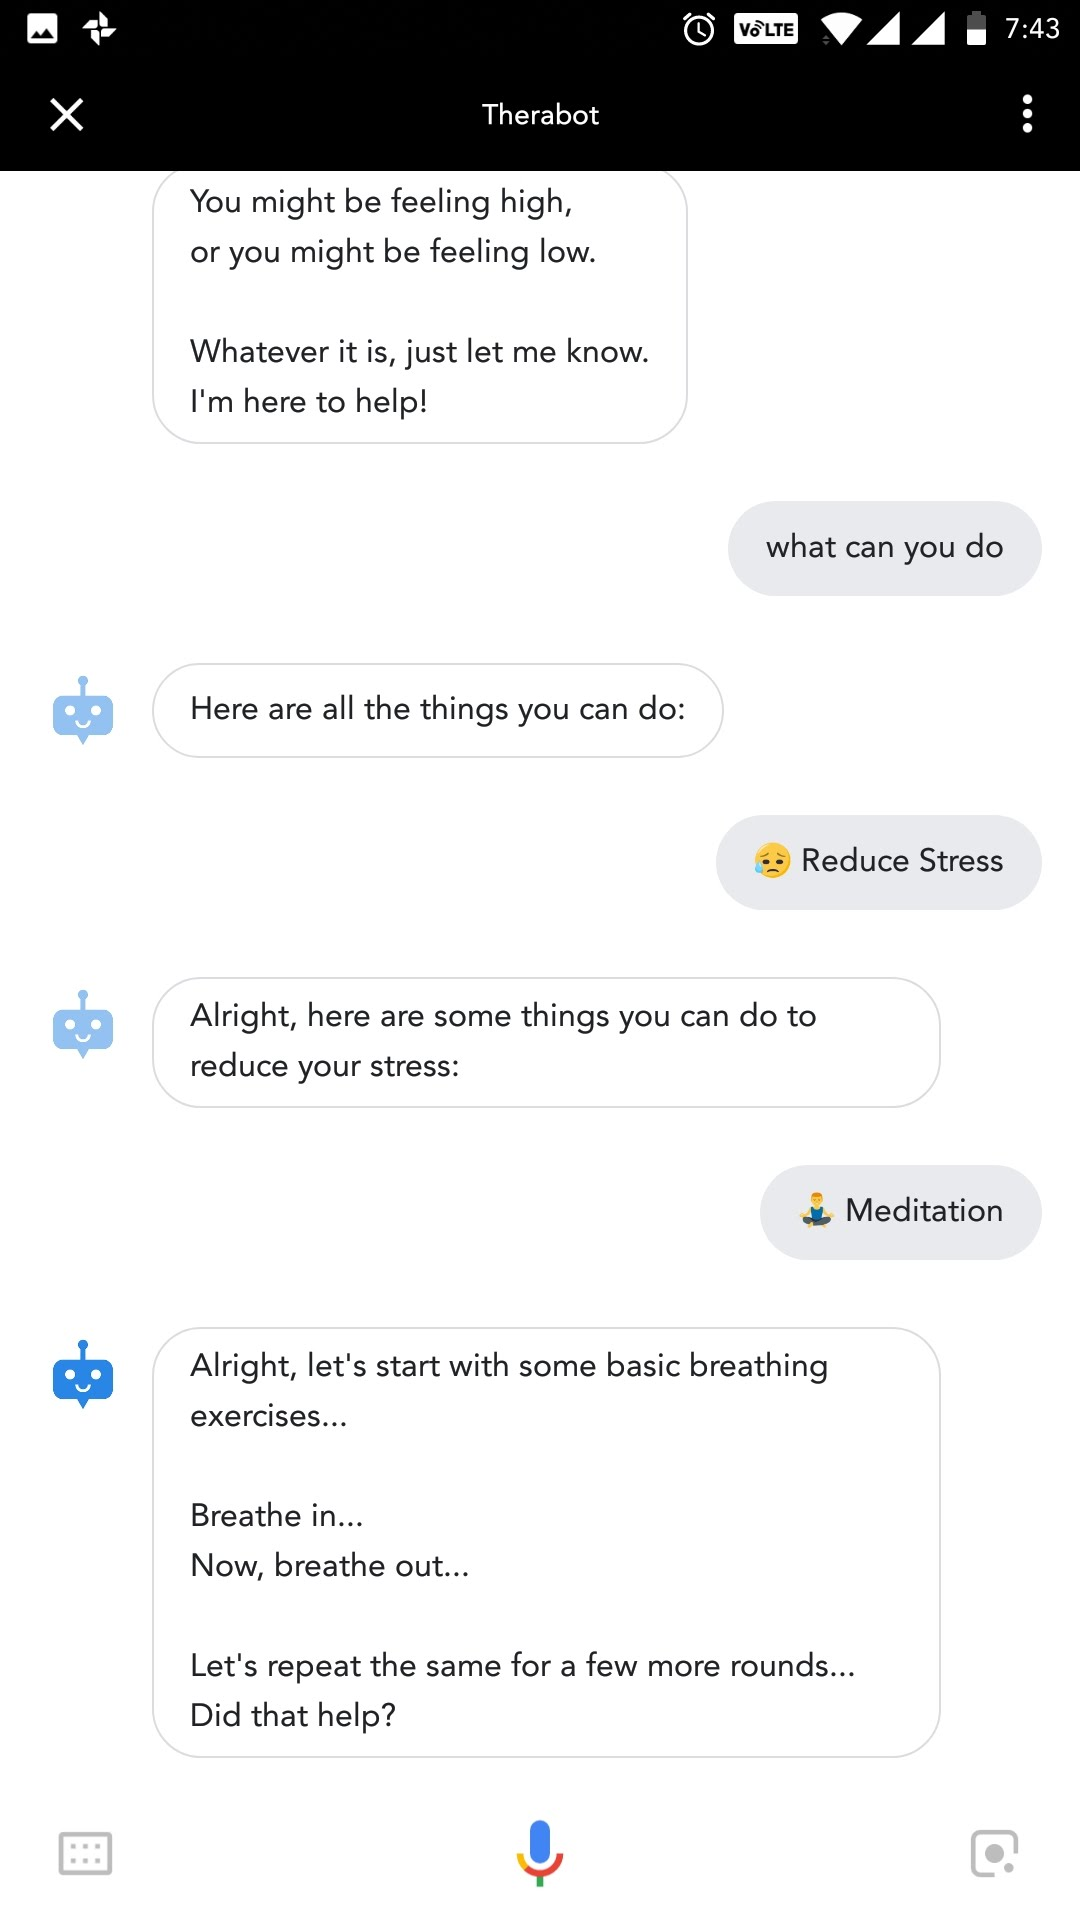
\includegraphics[width=0.9\textwidth]{screenshots/chatbot/7.jpg}
        \caption{Meditation w/ SSML}
    \end{minipage}\hfill
    \begin{minipage}{0.45\textwidth}
        \centering
        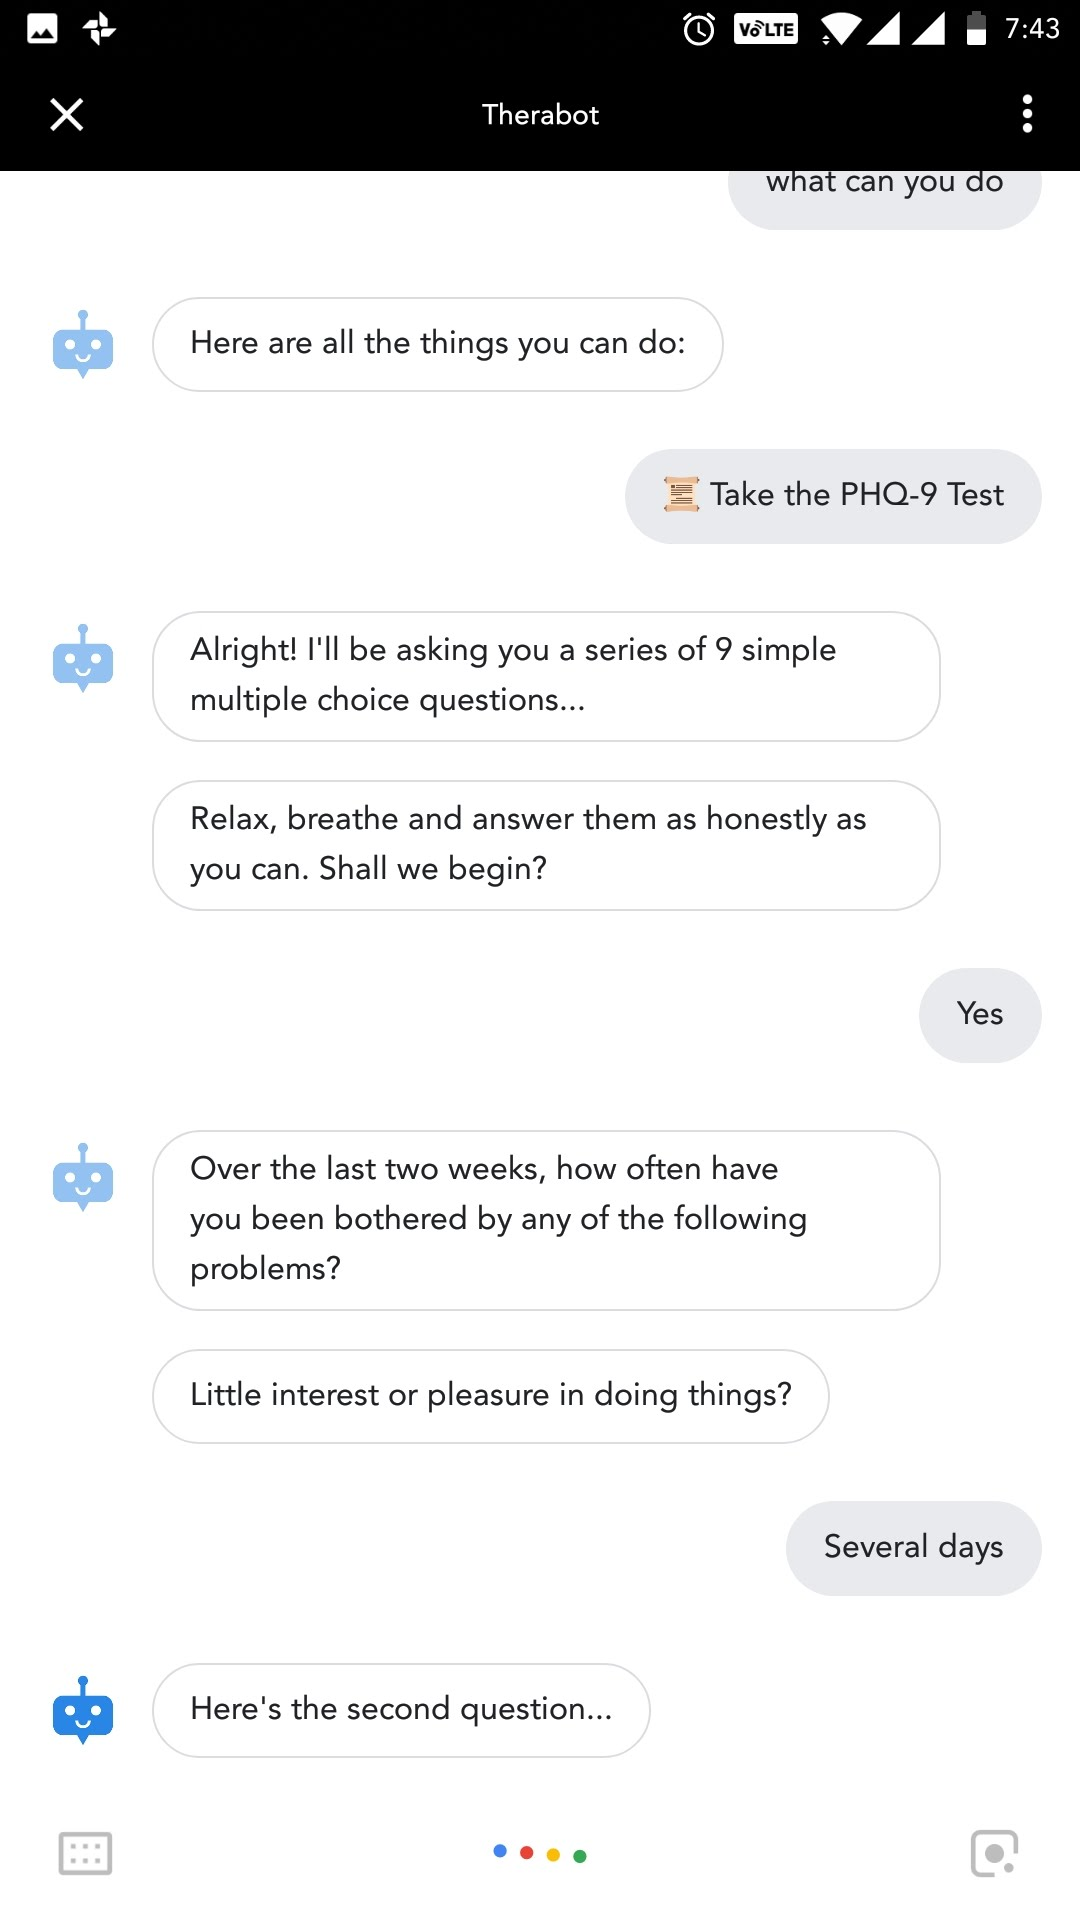
\includegraphics[width=0.9\textwidth]{screenshots/chatbot/8.jpg}
        \caption{PHQ9 Test}
    \end{minipage}
\end{figure}
\vspace*{\fill}

\pagebreak

\vspace*{\fill}
\begin{figure}[H]
    \centering
    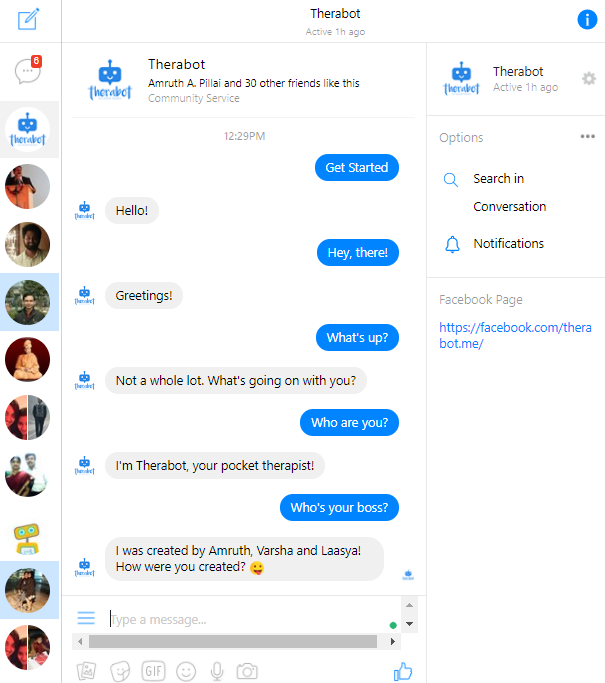
\includegraphics[width=12cm]{screenshots/chatbot/tablet.png}
    \caption{Tablet Screenshot}
\end{figure}

\begin{figure}[H]
    \centering
    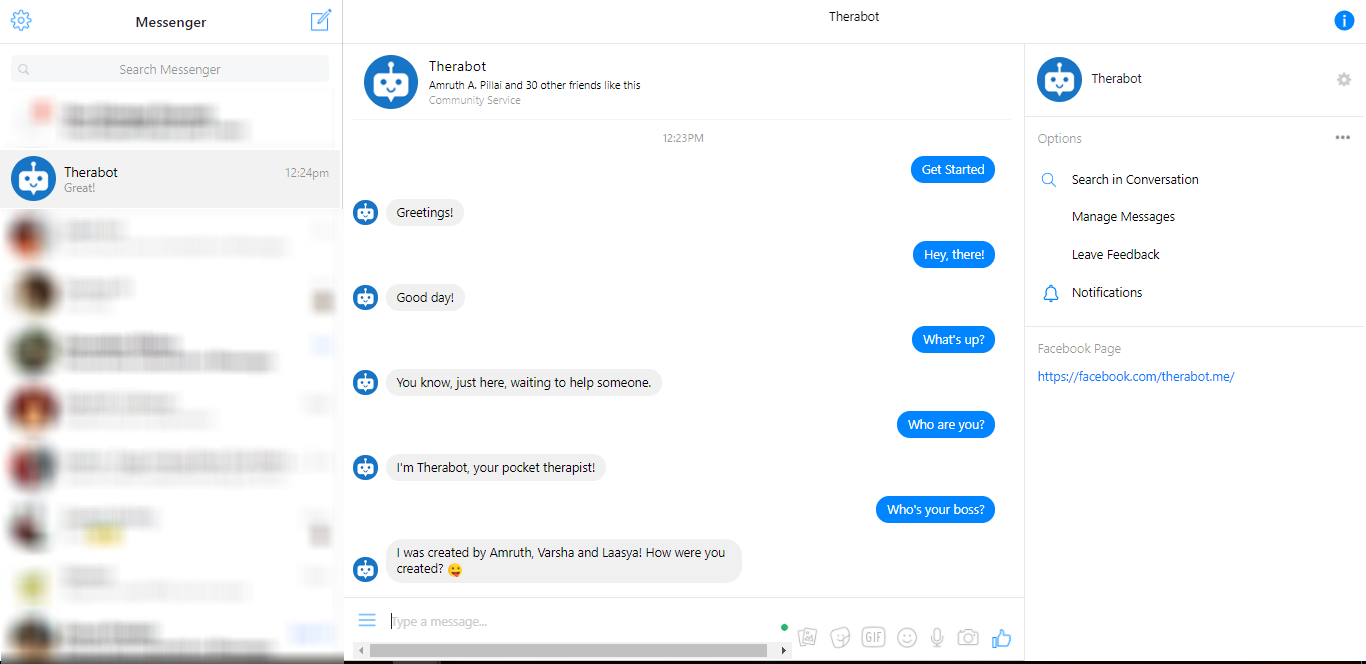
\includegraphics[width=\textwidth]{screenshots/chatbot/desktop.png}
    \caption{Desktop Screenshot}
\end{figure}
\vspace*{\fill}

\pagebreak

\section{Testing}

\subsection{Chatbot Testcases}

\noindent
We brought up our dataset of questions and answers and validated it across our testcases, it passed on all counts and can be verified by talking to the chatbot with the specified input parameters.

\begin{figure}[H]
    \centering
    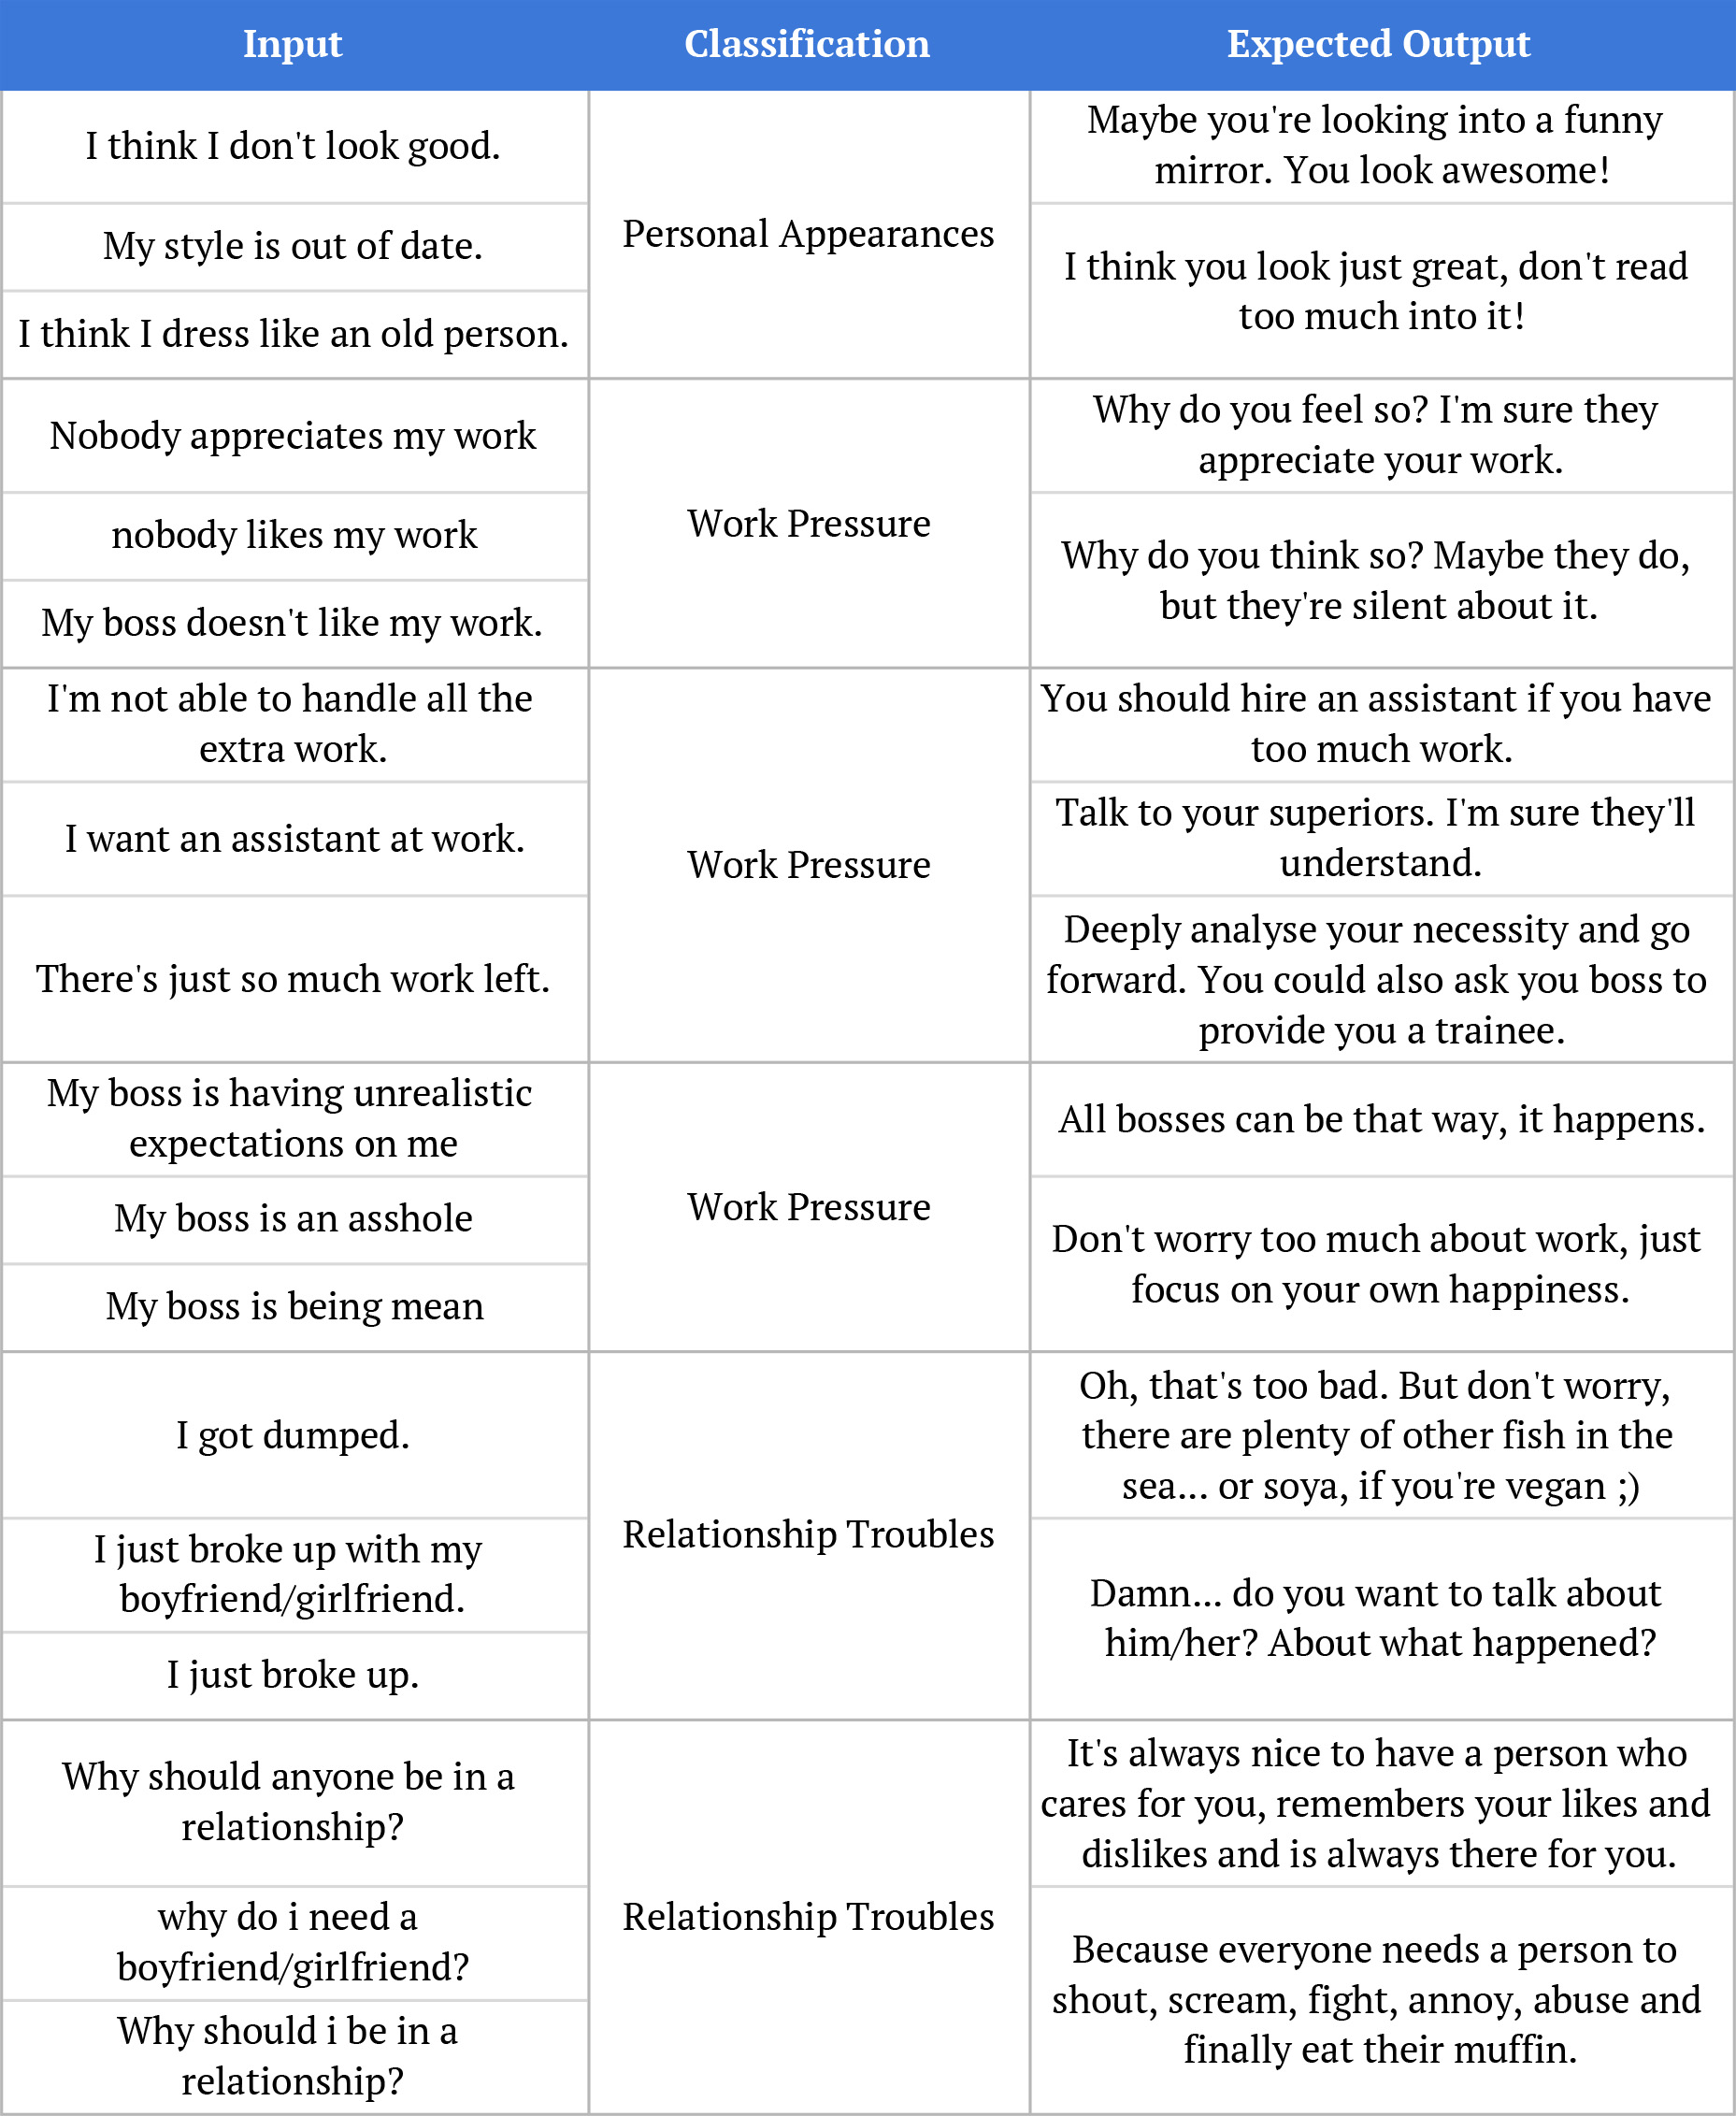
\includegraphics[width=\linewidth]{chatbot-testcases.jpg}
    \caption{Chatbot Testcases}
\end{figure}